\documentclass[a4paper,UTF8]{article}

\usepackage[margin=1.25in]{geometry}
\usepackage{color}
\usepackage{graphicx}
\usepackage{amssymb}
\usepackage{amsmath}
\usepackage{amsthm}
\usepackage{enumerate}
\usepackage{bm}
\usepackage{hyperref}
\usepackage{epsfig}
\usepackage{color}
\usepackage{mdframed}
\usepackage{lipsum}
\usepackage{mathtools}
\usepackage{algorithm}
\usepackage{algorithmic}
\usepackage{listings}
\usepackage{xcolor}
\usepackage{float}
\usepackage{caption}
\usepackage{mathrsfs}
\usepackage{amsmath}
\usepackage[utf8]{inputenc}
\usepackage[UTF8]{ctex}

\newmdtheoremenv{thm-box}{myThm}
\newmdtheoremenv{prop-box}{Proposition}
\newmdtheoremenv{def-box}{define}

\setlength{\evensidemargin}{.25in}
\setlength{\textwidth}{6in}
\setlength{\topmargin}{-0.5in}
\setlength{\topmargin}{-0.5in}

\usepackage{indentfirst}
\setlength{\parindent}{2em}

\usepackage{subfigure}
% \setlength{\textheight}{9.5in}
%%%%%%%%%%%%%%%%%%set header and footer here%%%%%%%%%%%%%%%%%%
\usepackage{fancyhdr}
\usepackage{lastpage}
\usepackage{layout}
\footskip = 10pt
\pagestyle{fancy}
\lhead{2020, Spring}
\chead{ }
\rhead{金庸的江湖——金庸武侠小说中的人物关系挖掘}
\cfoot{\thepage}
\renewcommand{\headrulewidth}{1pt}  			%header
\setlength{\skip\footins}{0.5cm}    			
\renewcommand{\footrulewidth}{0pt}  		

\makeatletter 							
\def\headrule{{\if@fancyplain\let\headrulewidth\plainheadrulewidth\fi%
\hrule\@height 1.0pt \@width\headwidth\vskip1pt	
\hrule\@height 0.5pt\@width\headwidth  			
\vskip-2\headrulewidth\vskip-1pt}      			
 \vspace{6mm}}     						
\makeatother

\graphicspath{{img/}}

\lstset{
 columns=fixed,
 basicstyle = \footnotesize,
 breakatwhitespace=false,         % 设置是否当且仅当在空白处自动中断.
 breaklines=true,
 numbers=left,                                        % 在左侧显示行号
 numberstyle=\tiny\color{gray},                       % 设定行号格式
 frame=none,                                          % 不显示背景边框
 backgroundcolor=\color[RGB]{245,245,244},            % 设定背景颜色
 keywordstyle=\color[RGB]{40,40,255},                 % 设定关键字颜色
 numberstyle=\footnotesize\color[RGB]{96,96,96},
 commentstyle=\color[RGB]{0,128,0},                % 设置代码注释的格式
 stringstyle=\rmfamily\slshape\color[RGB]{128,0,0},   % 设置字符串格式
 showstringspaces=false,                              % 不显示字符串中的空格
 language=JAVA,
 extendedchars=true,
 escapeinside=''                                       % 设置语言
}

%%%%%%%%%%%%%%%%%%%%%%%%%%%%%%%%%%%%%%%%%%%%%%
\numberwithin{equation}{section}
\newtheorem{myThm}{myThm}
\newtheorem*{myDef}{Definition}
\newtheorem*{mySol}{Solution}
\newtheorem*{myProof}{Proof}
\newcommand{\indep}{\rotatebox[origin=c]{90}{$\models$}}
\newcommand*\diff{\mathop{}\!\mathrm{d}}

\graphicspath{{img/}}

\usepackage{multirow}
\renewcommand\refname{reference}
\author{组长:韩畅,组员:李展烁、王一之、闫旭芃}
\begin{document}
%\listoffigures
\captionsetup[figure]{labelfont={bf},labelformat={default},labelsep=period,name={图}}
\title{金庸的江湖——金庸武侠小说中的人物关系挖掘}
\maketitle

\section{实验规划与设计}
\subsection{任务分配}
{171860551, \text{韩畅:组长,算法设计与实验规划,任务一、任务六,程序试运行与组织debug研讨}}\\ \indent
{171860550, \text{王一之:算法设计与实验规划,任务四,参与debug,实验版本控制}}\\ \indent
{171860549, \text{闫旭芃:算法设计与实验规划,任务五,参与debug与数据核对}}\\ \indent
{171840565, \text{李展烁:算法设计与实验规划,任务一优化、任务二、任务三,参与debug并提出重要优化思路}}
\subsection{任务要求}

\subsection{设计思路}


\section{实验实现}
\subsection{任务一:数据预处理}
\subsubsection{设计思路}
数据输入:已经分词、分段的多篇中文文本文件
\par 数据输出:每一段或几段中包含的所有人名,按顺序依次输出。
\par 需要注意的是,由于我们的实验是对金庸全部人物关系的分析,
因此无需特别地注意不同文件及文件名。
\par 我们使用提供的名单列表,通过HashSet结构,快速地比对词语
是否位于名单列表当中。
\par 在装载名单列表时,由于姓名数量的有限性,且由于
configuration只能传输字符串,
因此使用一个私有的将其全部装载到
一个字符串中,填入configuration中,
并在map的setup阶段将其提取出来,
并存储于HashSet中。
\par 特别地,为了提高效率,注意使用StringBuilder和String的相互配合。

\subsubsection{程序分析}
Main 主函数类:
\par 为了传递名单列表,调用NameLoader类的load方法,
从输入的文件名中获取名单,并使用configuration进行配置以备后用。
其余大多为路径、类名的配置,不赘述。如图\ref{task1-Main}
\begin{figure}[htbp]
    \centering
    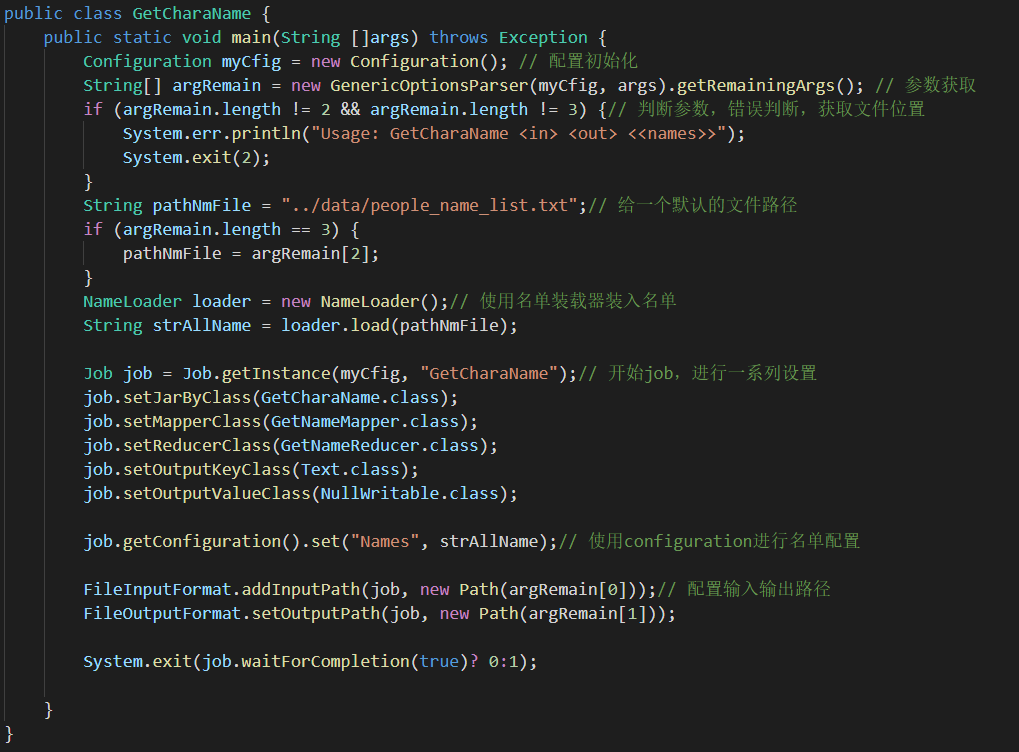
\includegraphics[width = 15cm]{task1-Main.png}
    \caption{主函数类具体实现}
    \label{task1-Main}
\end{figure}
\par NameLoader类:
\par 使用FileInputStream获取文件内容,使用BufferReader进行缓冲区文件读入操作。
\par 使用StringBuilder快速从单行读入中获取姓名,并快速构建字符串。如图\ref{task1-NameLoader}
\begin{figure}[htbp]
    \centering
    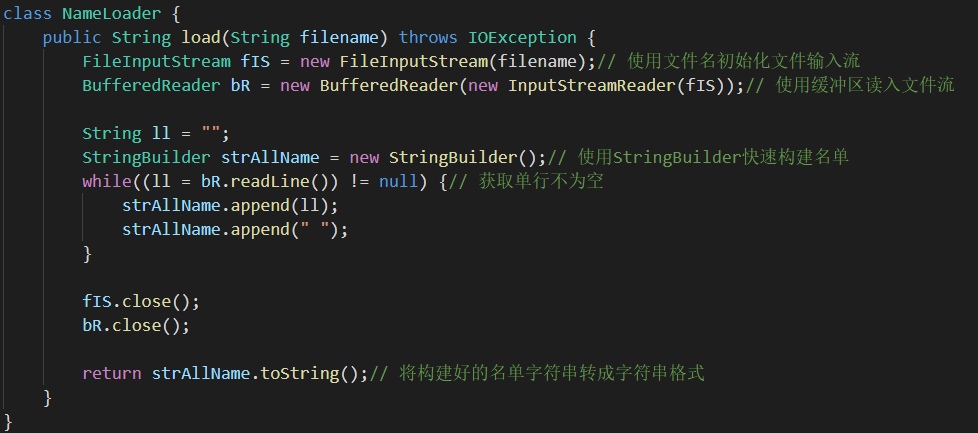
\includegraphics[width = 15cm]{task1-NameLoader.png}
    \caption{名单装载器具体实现}
    \label{task1-NameLoader}
\end{figure}

\par Mapper类:
\par 在setup中从configuration中获取之前装载的名单字符串,经过分词处理后,存入HashSet的名单表中。
\par 在map的重载函数中,对每行也即每个value值以空格为分隔符分割,并依此使用HashSet的查找操作比对是否属于姓名。并将姓名归并为一个字符串输出。如图\ref{task1-mapper}
\begin{figure}[htbp]
    \centering
    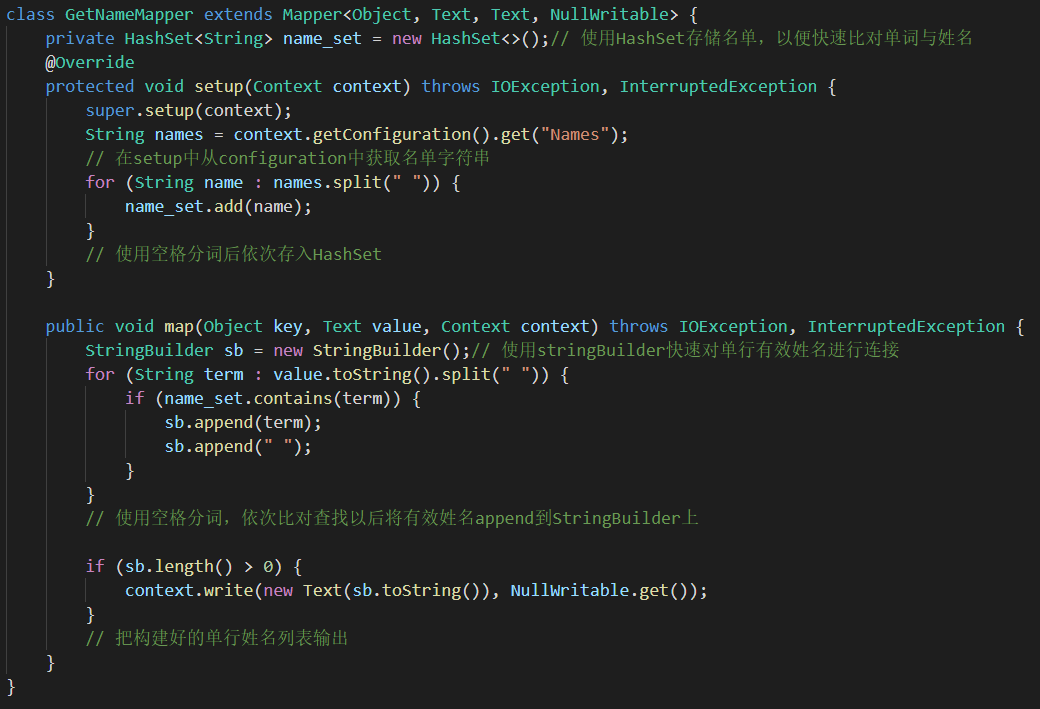
\includegraphics[width = 15cm]{task1-mapper.png}
    \caption{mapper具体实现}
    \label{task1-mapper}
\end{figure}

\par Reducer类:
\par 不做操作,直接将获取的值输出即可。

\subsection{任务二}
\subsubsection{设计思路}
\par 数据输入:每一段中包含的所有人名。
\par 数据输出:对于所有的段落,统计所有人名对出现在同一段落中的次数。
\par 使用IntWritable表示同现次数,因为同现次数在int可表示范围内。

\subsubsection{程序分析}
Main 主函数类:
\par 这里使用了reducer作为combiner,在mapper之后进行一次合并,减少传输数据量,作为优化。如图\ref{task2-Main}
\begin{figure}[htbp]
	\centering
	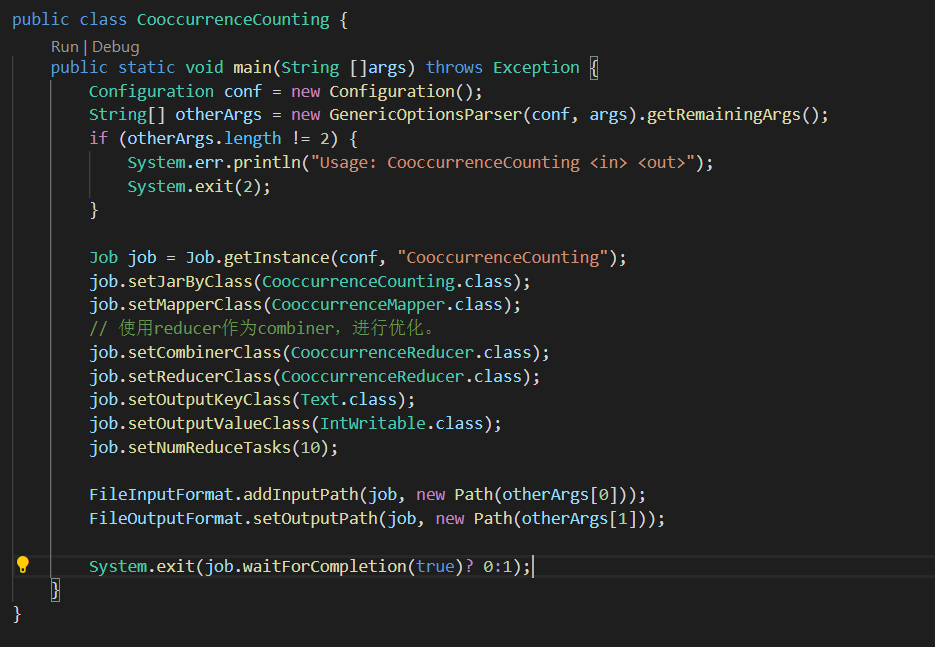
\includegraphics[width = 15cm]{task2-Main.png}
	\caption{主函数类具体实现}
	\label{task2-Main}
\end{figure}

\par Mapper类:
\par 使用HashSet来对于同一段落中所有人名进行去重。再使用双重for循环来发射所有两个不同人名构成的人名对。因为是在HashSet内遍历,这里判断两个String不相等,不需要使用Java的!equals()来判断String内容,只需要判断引用不同即可。如图\ref{task2-mapper}
\begin{figure}[htbp]
	\centering
	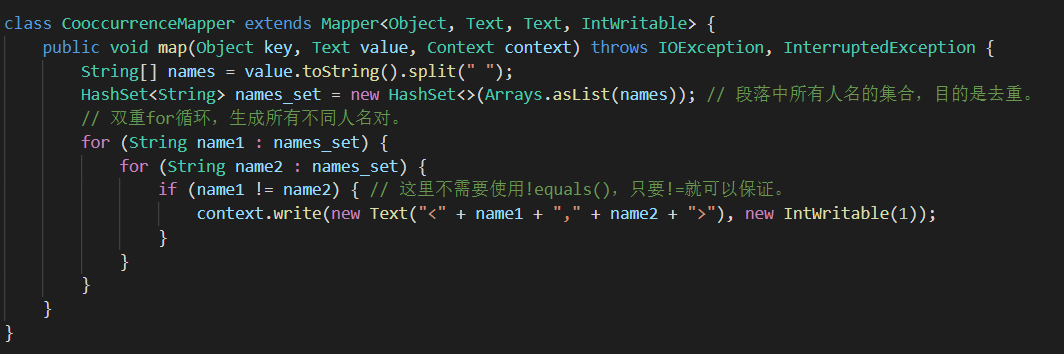
\includegraphics[width = 15cm]{task2-mapper.png}
	\caption{mapper具体实现}
	\label{task2-mapper}
\end{figure}

\par Reducer类:
\par 对于key对应的人名对出现次数进行求和。如图\ref{task2-reducer}
\begin{figure}[htbp]
	\centering
	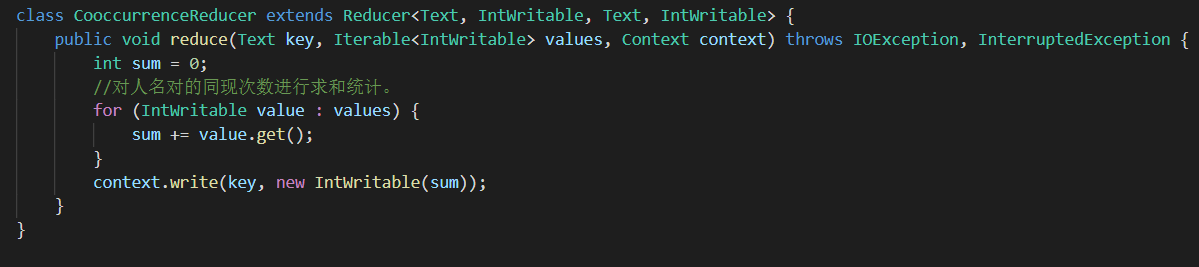
\includegraphics[width = 15cm]{task2-reducer.png}
	\caption{reducer具体实现}
	\label{task2-reducer}
\end{figure}
\subsection{任务三}
todo

\subsection{任务四:基于人物关系图的PageRank计算}
\subsubsection{PageRank算法介绍}
PageRank,又称网页排名,名字源于google创始人之一的Larry Page,是Google公司所使用的对与网页重要性排序的算法。\\
PageRank通过网页之间的超链接评价网页重要性,它的基本思想是:\\
\begin{enumerate}[1)]
    \item 如果一个网页被多个网页所指向,则该网页比较重要
    \item 如果一个重要的网页指向另一个网页,则另一个网页也比较重要
\end{enumerate}
该算法模拟一个上网者,随机打开一个网页,之后随机点击该网页的链接,统计上网者分布在每个网页的概率。\\
最初,每个网页的概率均等,每次跳转时,网页X将其PR(PageRank)均分到所指向的所有页面,记链接数为L(X),
于是,经过一次跳转后:\\
$$
PR(A)=\frac{PR(B)}{L(B)}+\frac{PR(C)}{L(C)}+\frac{PR(D)}{L(D)}+...
$$
我们将每个网页抽象成一个节点,超链接抽象为有向边,共同构成一个图。
则每次跳转可视为所有页面PR构成的特征向量R与该图的出度邻接矩阵M相乘,即:\\
$$R=
\begin{bmatrix}
    PR(p_1) \\
    PR(p_2)\\
    \vdots\\
    PR(p_n)\\
\end{bmatrix}
M=
\begin{bmatrix}
    p_1 \rightarrow p_1 & p_2 \rightarrow p_1 & \cdots & p_n \rightarrow p_1\\
    p_1 \rightarrow p_2 & p_2 \rightarrow p_2 & \cdots & p_n \rightarrow p_2\\
    \vdots & \vdots & \ddots & \vdots\\
    p_1 \rightarrow p_n & p_2 \rightarrow p_n & \cdots & p_n \rightarrow p_n\\
\end{bmatrix}
$$
\\
$$
R_1=M R_0
$$
多次迭代后,PR值趋于稳定,即为最终的PR值。

\subsubsection{设计思路}
任务四的输入为任务三的输出,格式如下:\\
人物 [名字$_1$,影响$_1$|名字$_2$,影响$_2$|...|名字$_n$,影响$_n$] \\
影响$_i$ 为 名字$_i$ 与该人物归一化后的同现次数,表示 名字$_i$ 对该人物的影响权重。\\
每个人物视为图的一个节点,边权重为二人同现次数。\\
对于普通的PageRank计算,由于会存在自环边以及无出度的节点,为方式到达某一节点后陷入该点,会加入“随机浏览者”(random surfer)的概念,
即到达某个节点后有一定概率直接跳转到任意一个节点,从而避免此情况。然而在此次任务中,首先没有自身与自身同现的情况,因此无自旋边;
同时A与B同现,则B一定与A也同现,因此不考虑权重时所有边实际都为无向边,因此不存在出度为0的节点。所以此次任务无需引入“随机浏览者”。\\

MapReduce框架下,运算分布进行,因此不使用邻接矩阵,而采用邻接表的形式。算法大致分为三阶段:\\

阶段一:预处理
首先要将输入格式化为供之后迭代处理的形式。采用如下格式:
key:人物\\
value:PageRank\#[名字$_1$,影响$_1$|名字$_2$,影响$_2$|...|名字$_n$,影响$_n$] \\
以概率为初始值,PageRank应设置为1/N,但N值较大,较小数字做乘法时误差较大,因此将初始PR设置为1来减小误差。\\

阶段二:迭代计算
迭代计算PR值,直到PR收敛。\\
在Mapper中,首先输出如下键值对:
key:人物\\
value:\#出度表\\
此对目的在于维护出度表,value前加\#使reducer便于区分。\\
记A的出度表集合为N,则A的新PR计算过程如下式:
$$
NewPR(A)=\sum_{x\in N}OldPR(x)*weight(x\rightarrow A)
$$
但此处不清楚N中其他任务的PR值,无法计算A的新PR,但由于同现关系构成的图为无向图,我们可以根据此关系计算A对N中所有人的影响,之后在Reduce阶段汇总即可。
因此生成如下键值对:\\
key:受影响人物\\
value:受影响值\\
在Reducer中,首先查看value前是否有\#号以区分该键值对类型。之后将受影响值累加得到新PR值。\\
由于是一个迭代过程,将输出格式化,与Mapper的输入格式相同。\\

阶段三:处理结果
在Mapper阶段去除结果中的出度表,只保留PR值。\\
利用Partition类进行排序,由于默认为升序,结果需要降序,因此重写DoubleWritable。
因为只有1000余数据,未采用采样排序,使用了简单的全排序。\\
Reducer阶段整理输出即可

\subsubsection{代码讲解}
程序可分为三个模块:PageRank、RageResultSort以及调度模块。\\\\

模块一:PageRank\\
此模块实现了了阶段一与阶段二的任务。
\begin{figure}[H]
    \centering
    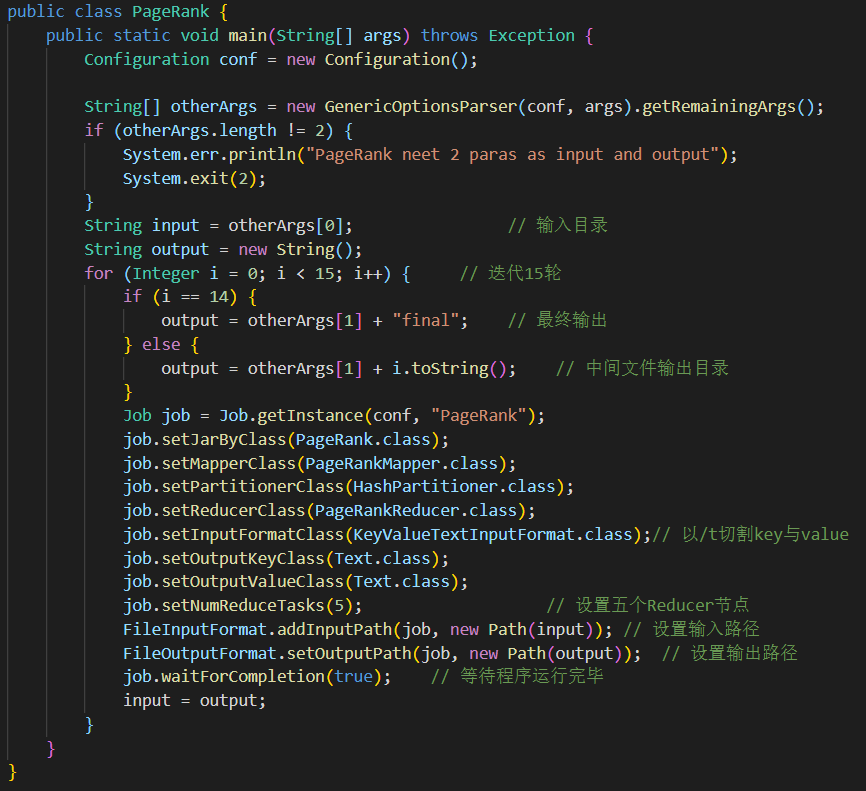
\includegraphics[width = 15cm]{PageRankMain.png}
    \caption{PageRankMain}
    \label{PageRankMain}
\end{figure}
图\ref{PageRankMain}为此类的main函数,使job运行15次,每次的结果储存在以运行次数为名的文件夹内,
下一次迭代的输入为上一次的输出。最终结果储存在“final”文件夹下。由于程序中用不到行号,设置InputFormat为KeyValueTextInputFormat,
这样会自动以分隔符(默认为$\backslash$t)将一行的内容切割为key和value。\\
\begin{figure}[H]
    \centering
    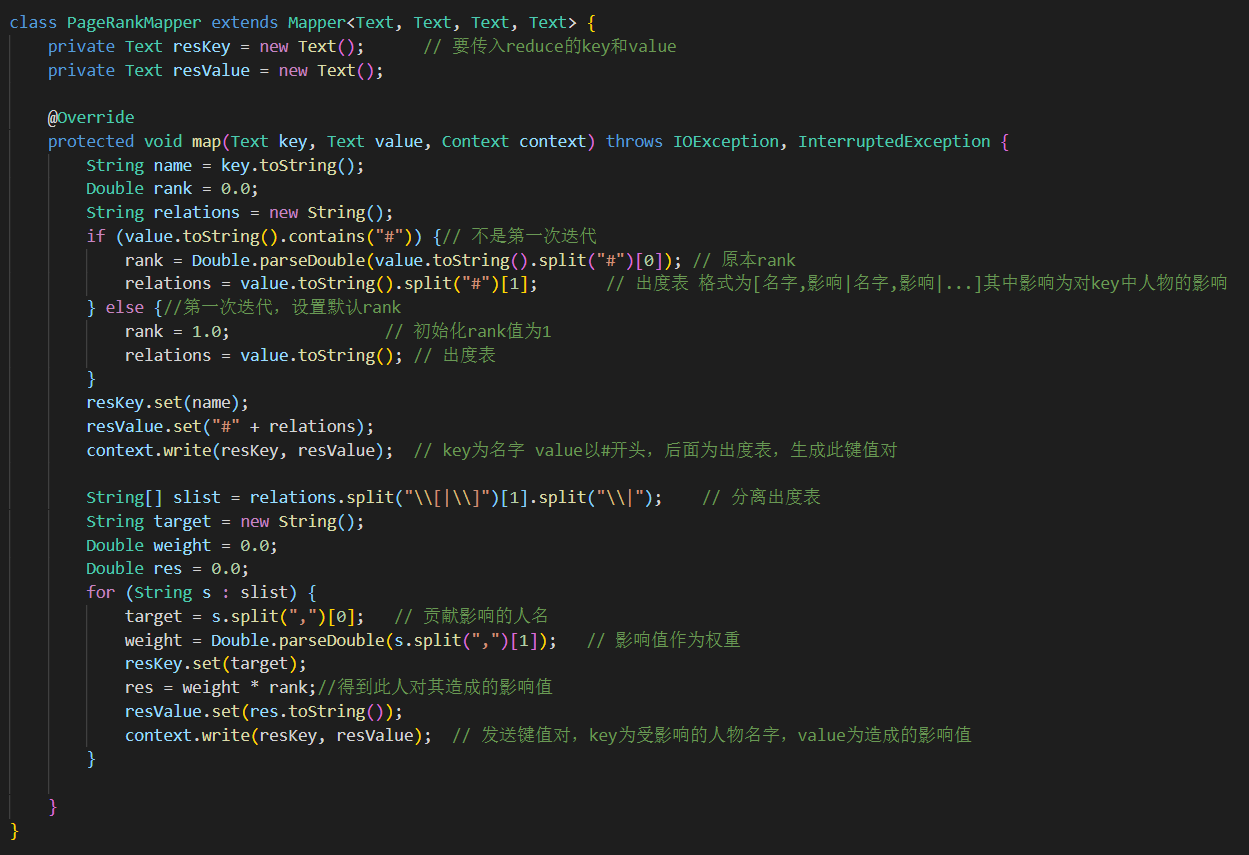
\includegraphics[width = 15cm]{PageRankMapper.png}
    \caption{PageRankMapper}
    \label{PageRankMapper}
\end{figure}
图\ref{PageRankMapper}为Mapper函数,此阶段,首先通过value中是否有\#号来判断是否是第一次迭代。
若为不为第一次,提取之前的RP,否则设置默认的PR值为1.0。通过value中的出度表,计算新PR值。向reducer发送“姓名 \#出度表”
以及“姓名 PR值”两个键值对。\\
\begin{figure}[H]
    \centering
    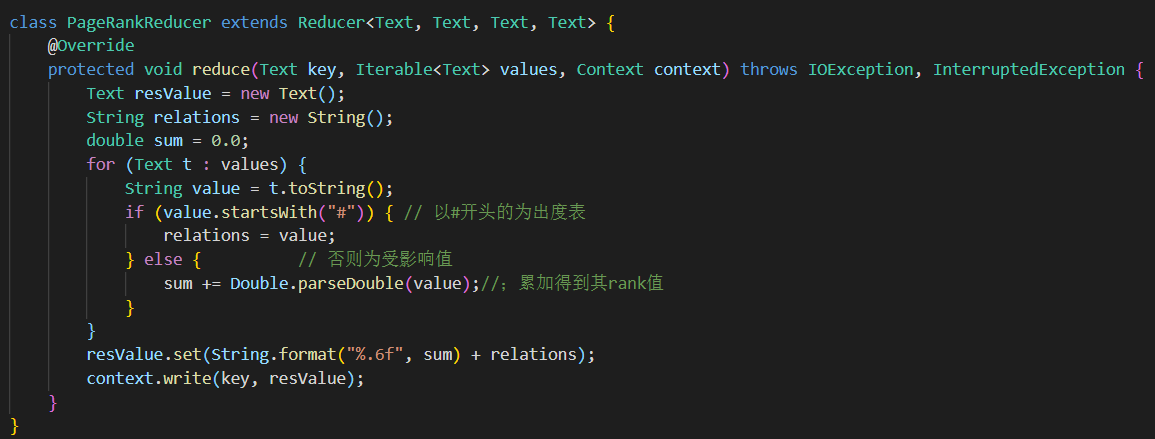
\includegraphics[width = 15cm]{PageRankReducer.png}
    \caption{PageRankReducer}
    \label{PageRankReducer}
\end{figure}
图\ref{PageRankReducer}为Reducer函数,通过\#判断键值对类型,合并格式化后输出。\\\\

模块二:PageResultSort\\
此模块实现了阶段三的任务。\\
main函数中同样设置InputFormat为KeyValueTextInputFormat,同时设置reducer数量为1。
\begin{figure}[H]
    \centering
    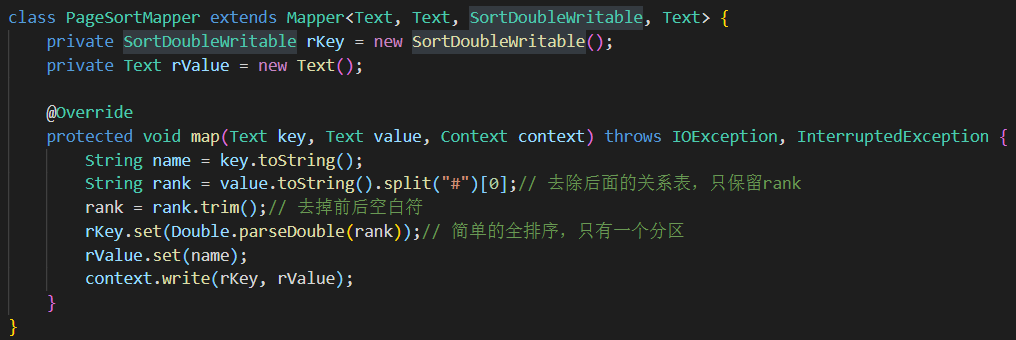
\includegraphics[width = 15cm]{PageSortMapper.png}
    \caption{PageSortMapper}
    \label{PageSortMapper}
\end{figure}
图\ref{PageSortMapper}为Mapper函数,去除不需要的出度表。为进行排序,将PR值作为key,名字作为value。
\begin{figure}[H]
    \centering
    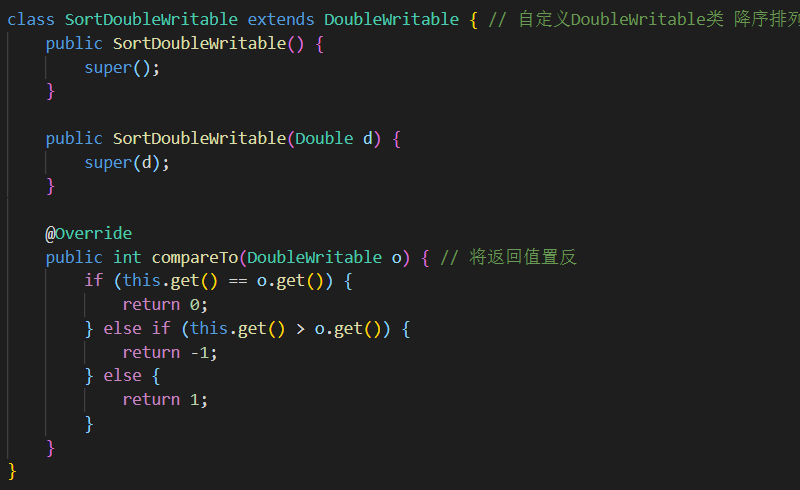
\includegraphics[width = 15cm]{SortDoubleWritable.png}
    \caption{SortDoubleWritable}
    \label{SortDoubleWritable}
\end{figure}
\begin{figure}[H]
    \centering
    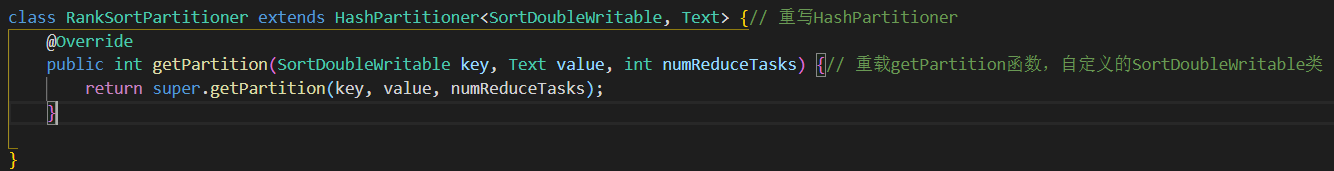
\includegraphics[width = 15cm]{RankSortPartitioner.png}
    \caption{RankSortPartitioner}
    \label{RankSortPartitioner}
\end{figure}
图\ref{RankSortPartitioner}与图\ref{SortDoubleWritable}为重载的Partitioner函数以及SortDoubleWritable类。
重载Partitioner函数使得以DoubleWritable类型的key进行排序,由于默认DoubleWritable为升序,重载DoubleWritable为自定义SortDoubleWritable进行降序排列。
\begin{figure}[H]
    \centering
    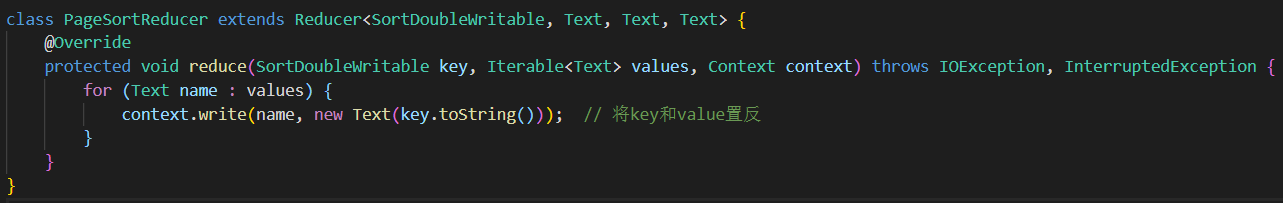
\includegraphics[width = 15cm]{PageSortReducer.png}
    \caption{PageSortReducer}
    \label{PageSortReducer}
\end{figure}
图\ref{PageSortReducer}为Ruducer,将key与value互换位置,保证输出时名字在前。

\subsection{任务五:在人物关系图上的标签传播}
思路分析:在本实验里,我们拟采用 LPA(Label Propagation Algorithm) 标签传播算法对金庸小说中的人物进行聚类。 LPA 是一种半监督的图分析算法,能够为图中的每一个节点打上标签,对图的顶点进行聚类,从而在一张类似社交网络的图中完成社区发现。
\subsubsection{LPA算法介绍}
\textbf{算法思路:}\par
对于网络中的每一个节点,在初始阶段,Label Propagation算法对于每一个节点都会初始化一个唯一的一个标签。每一次迭代都会根据与自己相连的节点所属的标签改变自己的标签,更改的原则是选择与其相连的节点中所属标签最多的社区标签为自己的社区标签,这就是标签传播的含义了。随着社区标签不断传播。最终,连接紧密的节点将有共同的标签。\par
\textbf{算法过程:}\\
第一步:先给每个节点分配对应标签,即节点1对应标签1,节点i对应标签i;\\
第二步:遍历N个节点(for i=1:N),找到对应节点邻居,获取此节点邻居标签,找到出现次数最大标签,若出现次数最多标签不止一个,则随机选择一个标签替换成此节点标签;\\
第三步:若本轮标签重标记后,节点标签不再变化(或者达到设定的最大迭代次数),则迭代停止,否则重复第二步\\
具体伪代码如下图:
\begin{figure}[H]
    \centering

    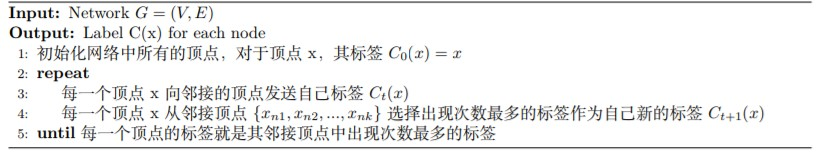
\includegraphics[width = 15cm]{LPAcode.jpg}

    \caption{LPA算法伪代码}
\end{figure}
对于金庸小说中的人物关系的标签分析来说,其中人物的网络可以看成一个每条边带权值的有向图,因此我们的算法也要在此基础上做一些改变。首先我们还是对每一个顶点进行初始化,然后每一个顶点根据自己的出边向邻接顶点发送自己的标签。最后每个顶点从自己收到的标签里取权值和最大的标签作为自己新的标签(原算法的出现次数之和需要改成权值之和),相当于原算法中。当每一个顶点 的标签不再改变时,算法终止。\par
具体分为3个部分进行: 
\subsubsection{第一部分: LabelInitial 社区初始化}
第一个阶段,初始化每一个顶点,将每一个节点的人物姓名作为该节点的标签。(人名,(标签\#邻接表))\par
Map:一行一行分析实验三的输出结果,直接将每个顶点的人名作为每个顶点的标签,输出  \par
Reduce:不做任何处理直接输出 (人名,(标签\#邻接表))\par
\textbf{Mapper类:}\par
一行行读入任务三输出的结果 ( 人名,邻接表 ),然后将人名作为该任务的标签以 ( 人名,(标签,邻接表)) 的形式输出。初始时,每一个节点都是一个独立的社区,所以这里直接将标签赋值成该节点的人物姓名即可\\
\begin{figure}[H]
    \centering

    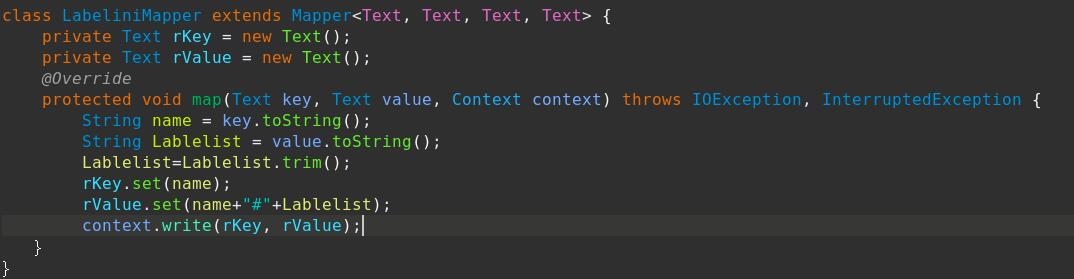
\includegraphics[width = 15cm]{5-1mapper.jpg}

    \caption{LabelInitial Mapper}
\end{figure}

\textbf{Reduce类:}\par
直接输出即可,同时在main函数中设置job.setNumReduceTasks=1输出一个文件即可\\

\subsubsection{第二部分:LabelAnalyse LPA社区聚类迭代}
第二个阶段,读入第一部分处理好的数据,分别发送邻接表(节点,邻接表)和每一条边(即(节点的邻居人名,节点标签:二者所连边的权重)),之后利用相同key将同一个节点和不同标签的边分在同一个reducer的同一个组里面,之后选择出现权重和最大的标签作为新的标签即可。之后累次循环迭代直到标签稳定。\par
同时,LPA当遇到二分图的时候,会出现标签震荡,这里当迭代轮数超过 10 轮后就会开始震荡,因此我们这里可以选择迭代 15 -20轮。\par

\textbf{伪代码:}\par
\begin{figure}[H]
    \centering

    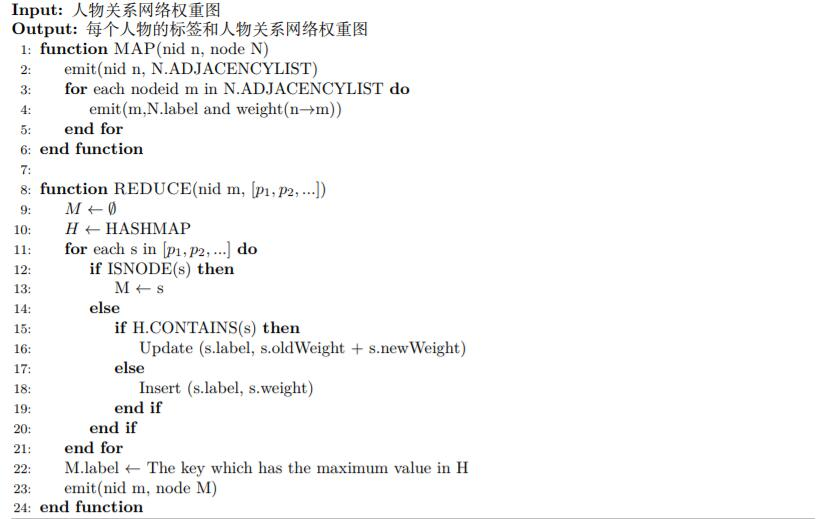
\includegraphics[width = 15cm]{5-2code.jpg}

    \caption{LabelAnalyse伪代码}
\end{figure}
\paragraph{具体程序:}
\subparagraph{1. Mapper类:}
\par 首先读入第一部初始化好的数据,首先发送(原节点人名,\#邻接表)用于维护每一个节点的网络结构,以便下一次迭代使用
\par 然后拆开邻接表中每一个邻居节点,将邻居节点姓名作为key,将该节点标签和权值作为value,发送(节点的邻居人名,节点标签:二者所连边的权重)
\begin{figure}[H]
    \centering

    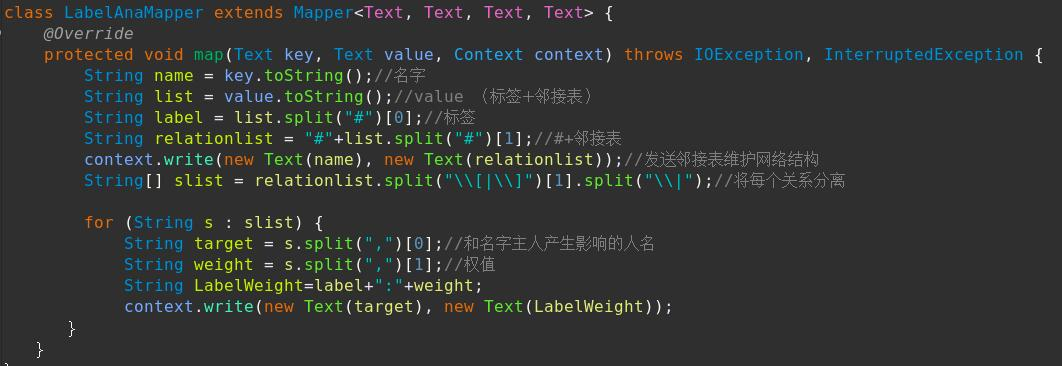
\includegraphics[width = 15cm]{5-2MAPPER.jpg}

    \caption{LabelAnalyse Mapper}
\end{figure}
\subparagraph{1. Reducer类:}
\par 当读入 ( 人名, \#邻接表 )时,直接保存邻接表维护网络结构,以便下一次迭代使用。
\par 当读入(节点的邻居人名,节点标签:二者所连边的权重)时,首先创建一个HashMap 数据结构,维护每一个(标签,权重),循环读入所有的这种输入。如果收到的该标签还没有出现过,那么以标签为key,权值为value插入哈希表中。如果标签已经出现过,则标签权值在原来的权值基础上累加上去。
\par 然后循环比较,取权值和最大的标签作为新的标签,还是以原来的格式(节点名称,标签\#邻接表) 输出作为结果
\begin{figure}[H]
    \centering

    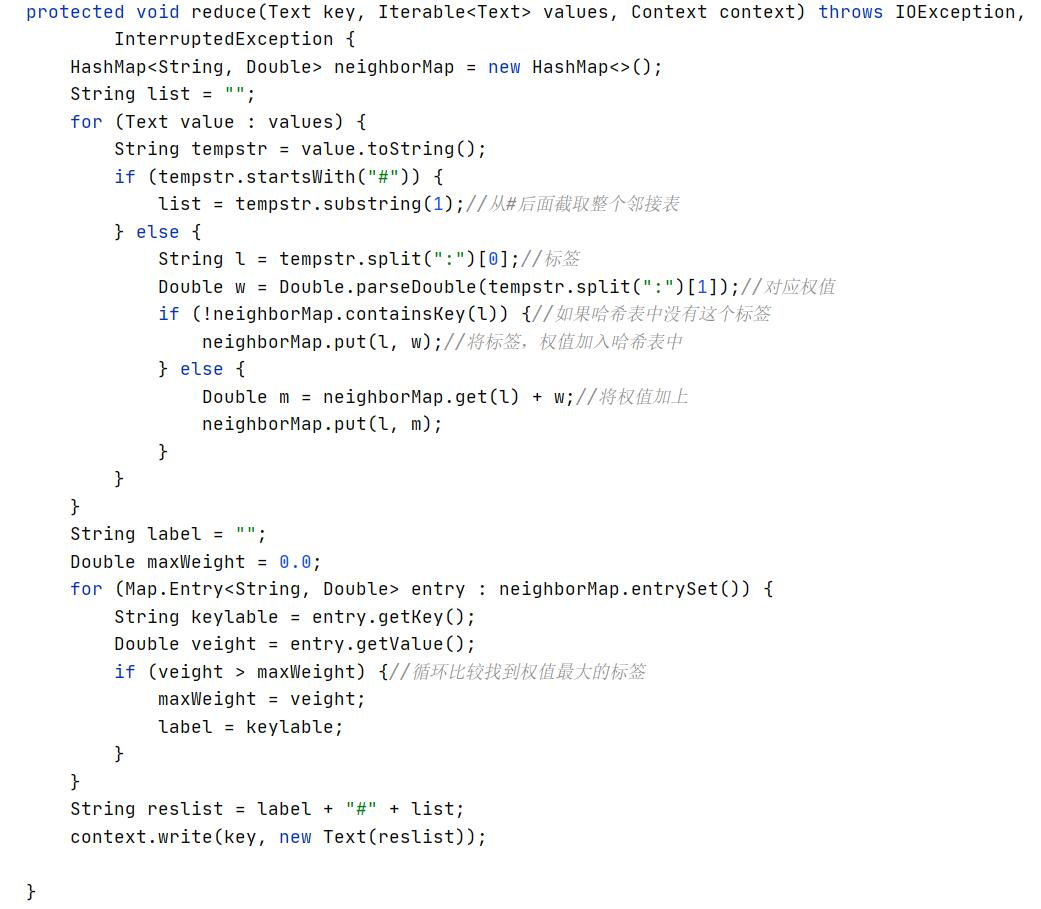
\includegraphics[width = 15cm]{5-2reducer.jpg}

    \caption{LabelAnalyse Reducer}
\end{figure}
\subparagraph{1. Main函数:}
设置一个循环即可,循环20次,每次的输出变成下一次的输入
\begin{figure}[H]
    \centering

    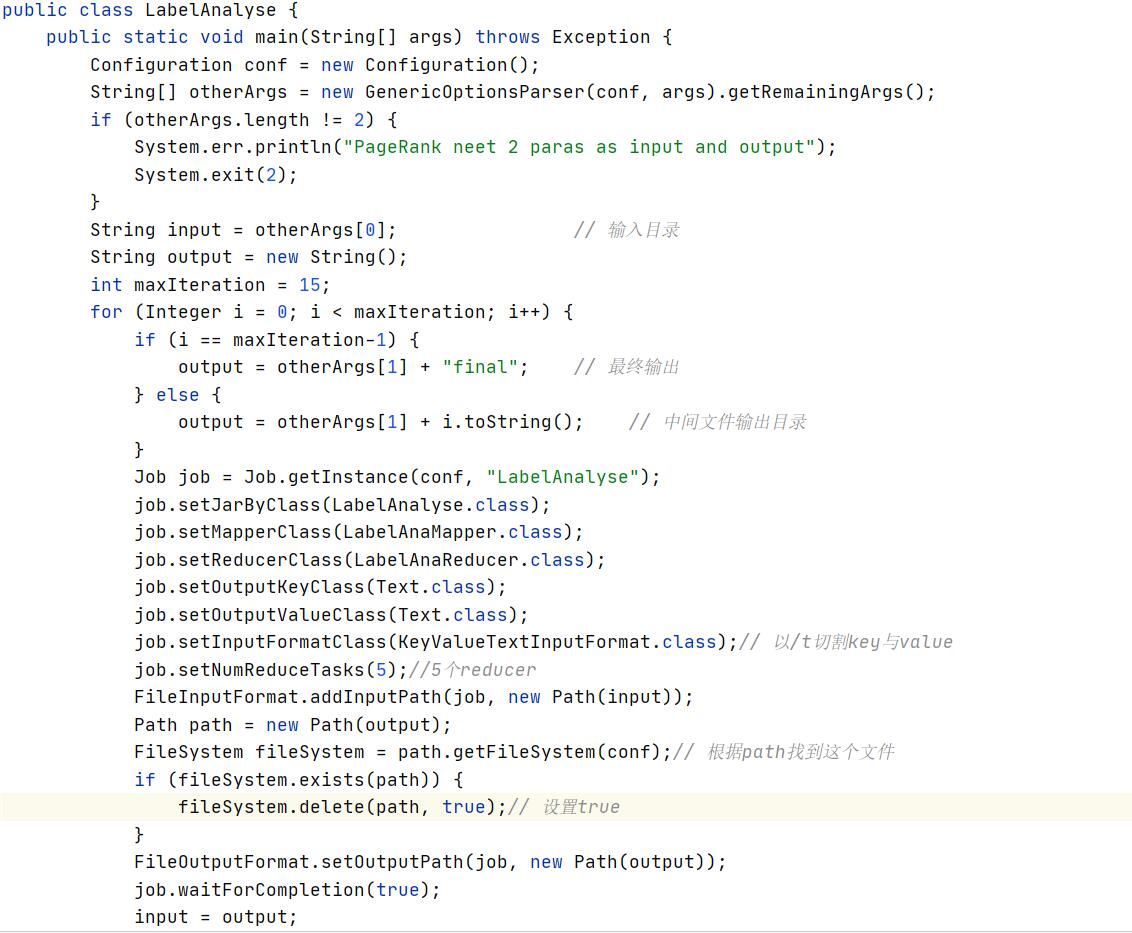
\includegraphics[width = 15cm]{5-2main.jpg}

    \caption{LabelAnalyse Main函数}
\end{figure}
\subsubsection{第三部分:LabelResult 结果整理(包括任务六的一部分)}
\par 这里因为第二部分输出的结果中还有邻接表的存在,而且结果比较杂乱,所以直接将任务六数据整理整合到这一部分。在mapper中读入(节点名,标签\#邻接表),去除邻接表,并且将标签和节点名反转,将标签设置成key,输出(标签,节点名)以便之后归类
\par 其中重写了partition类,将首字母拼音在a-h,h-p,p-z分为三个区域,分三个文件存储,这个功能可加可不加,如果不加的话那么就输出一个文件,文件中相同标签会在一起,比较直观。
\par reducer部分直接输出((标签,人名),空)
\begin{figure}[H]
    \centering
    \subfigure[LabelResult Mapper]
	{
		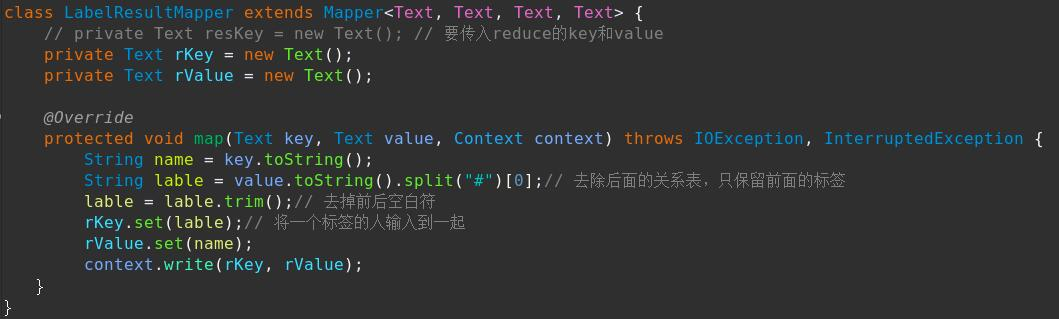
\includegraphics[width = 15cm]{5-3mapper.jpg}
	}
	\vfill
	\subfigure[LabelResult Reducer]
	{
		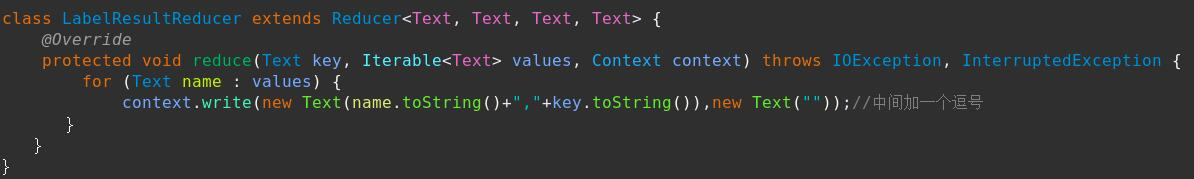
\includegraphics[width = 15cm]{5-3reducer.jpg}
	}
	\vfill
	\subfigure[LabelResult Partitioner]
	{
		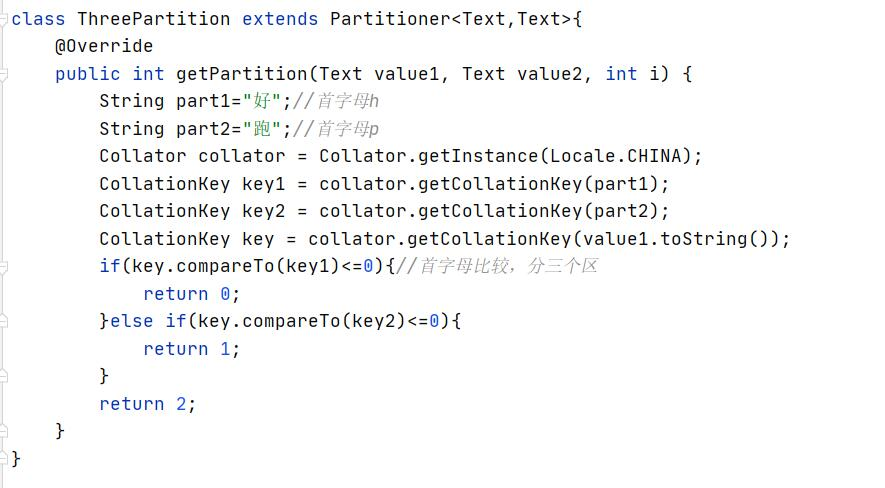
\includegraphics[width = 15cm]{5-3partitioner.jpg}
	}
	
	\caption{LabelResult 部分代码截图}
\end{figure}
\subsubsection{总结:}
\paragraph{LPA算法优点:}
\par LPA算法的最大的优点就是算法的逻辑非常简单,相对于优化模块度算法的过程是非常快的,不用pylouvain那样的多次迭代优化过程。
\par LPA算法利用自身的网络的结构指导标签传播,这个过程是无需任何的任何的优化函数,而且算法初始化之前是不需要知道社区的个数的,随着算法迭代最后可以自己知道最终有多少个社区
利用MapReduce可以很好的利用其特性来进行迭代分析
\paragraph{LPA算法缺点:}
\par 划分结果不稳定,随机性强是这个算法致命的缺点。具体体现在:
\subparagraph{1. 更新顺序:}
节点标签更新顺序随机,但是很明显,越重要的节点越早更新会加速收敛过程;
\subparagraph{2. 随机选择:}
如果一个节点的出现次数最大的邻居标签不止一个时,随机选择一个标签作为自己标签。这种随机性可能会带来一个雪崩效应,即刚开始一个小小的聚类错误会不断被放大。不过如果相似邻居节点出现多个,可能是权重weight计算的逻辑有问题,需要回过头去优化weight抽象和计算逻辑;

\subsection{任务六:基于PageRank的可视化}
\subsubsection{设计思路}
金庸的全部武侠小说中总共包含人物一千余名,其存在的相互关联可能达到100K的等级,
在这样庞杂的人物关系中,想要让全部的人物和关系呈现在受众面前,是不现实的。
这一判断得到了很多前车之鉴的证实,例如使用gephi软件生成的关系图,如同一团乱麻,
几乎看不清任何的姓名或关系,更枉谈“得到一些有趣的结论”。
\par 在这样的前提下,我们选择了对可视化的内容进行取舍,将可视化的人物数量级从1000降低
到了100的量级。同时对人物的重要性、人物关系的亲密度以PageRank及其排序的结果
进行刻画,从而得到了比较好的视觉效果。
\par 为了进行个性化的开发,我们选择了Qt作为可视化部分的开发平台,使用C++作为开发语言,
编写了一个RelationPainter的程序,对数据进行个性化的、延拓性强的可视化操作。
利用该程序,我们可以
\begin{itemize}
    \item 通过文件装载按钮,使用txt文件作为输入,直接获得效果图;
    \item 通过关系曲线的粗细更直观地表示了人物关系的亲密程度;
    \item 通过人物姓名和标识点的尺寸,可以更直观地感受人物的重要性;
    \item 通过关系曲线的颜色,更清晰地辨别同一个人所具有的人物关系;
    \item 通过关系曲线的高亮,更快地辨别某一特定个体的关系网;
    \item 通过操控“显示最重要的n位人物”拖动条,控制显示在视野中的人数;
    \item 通过操控“调整显示尺寸”拖动条,控制人物关系显示的疏密程度,从而避免人物的重叠;
    \item 通过将人物名称和人物标识点围成圆环状,避免了姓名与人物关系线条的重叠。
\end{itemize}
该程序的上限很高,延拓性很广,我们将在后面相关章节中详细介绍其改进和优化思路。

\subsubsection{程序分析}
Relation 类:
\par 这是一个刻画单个人物及与之相关的人物关系的类。
其中,通过QList<QPair<QString,double>>
维护了一个人物关系表,从而可以对于该人物相关的
人物关系进行操作。如图\ref{task6-Relation}
\begin{figure}[htbp]
    \centering
    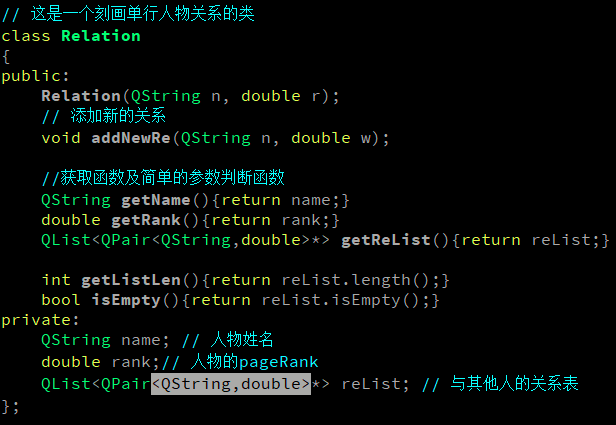
\includegraphics[width = 15cm]{task6-Relation.png}
    \caption{单人物关系类具体实现}
    \label{task6-Relation}
\end{figure}

\par sigFig 类:
\par 这是一个以单人物关系为基础的单图元类。
在这个类中,维护了一个Relation类对象以存储人物关系。
同时根据其中图元绘制参数常量的值,在绘制之前更新其图元的
各项属性(如粗细、颜色、大小、角度、位置、透明度等),
之后通过其中的绘制函数分别绘制人物标志点、人物名和人物关系曲线。
一般来说,人物的PageRank值越高,人物名和标志点绘制得
就越大越粗,而人物关系的权重越高,人物关系曲线就绘制得越粗。
\par 特别的,由于我们将人物标志点和人物名
绘制成圆盘状以避免重叠,而每个人物又在圆盘上
占据不同的角度值,因此需要给每个人物图元在绘制前计算
其在圆盘所占的角度。又因为每个单图元类没有其他图元的角度信息,
因此在绘制关系曲线的时候,需要在更高层的类计算好
角度对应表,并传入关系曲线的绘制函数。

\par 由于类中大部分的方法为更新参数、获取
或设置变量的方法,故不做展示,只集中展示
genAll(更新所有参数),paintDot(绘制标志点),
和paintLine(绘制标志曲线)三个函数的实现。

\begin{figure}[htbp]
    \centering
    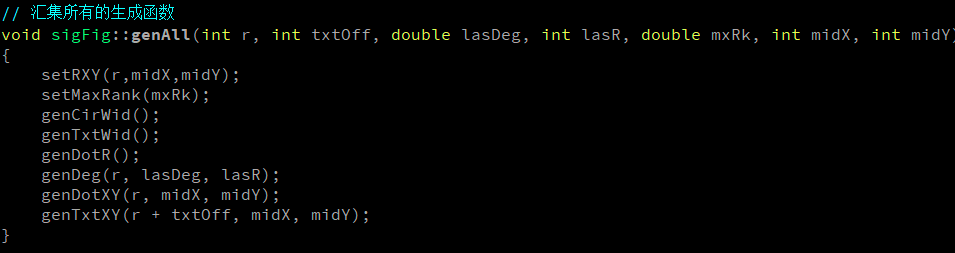
\includegraphics[width = 15cm]{task6-sigFig-genAll.png}
    \caption{单图元,全参数更新函数具体实现}
    \label{task6-sigFig-genAll}
\end{figure}
在图\ref{task6-sigFig-genAll}中,我们看到,
在对r(圆盘半径),midX、midY(屏幕中心X、y),mxRk(最大的PageRank值)
设置过后,分别对CirWid(标志点粗细)、TxtWid(人物名粗细)、
DotR(标志点大小)、Deg(标志点角度)、DotXY(标志点坐标)、
TxtXY(人物名坐标)进行了更新。
\begin{figure}[htbp]
    \centering
    \includegraphics[width = 15cm]{task6-sigFig-PaintDot.png}
    \caption{单图元,绘制标志点函数具体实现}
    \label{task6-sigFig-PaintDot}
\end{figure}
在图\ref{task6-sigFig-PaintDot}可以看到,在更新了全部的绘制
参数后,使用Qpainter、QPen、QFont等变量对画笔进行了设置,
将画笔移动一定的角度和坐标,并依此绘制圆和Text文本。
\begin{figure}[htbp]
    \centering
    \includegraphics[width = 15cm]{task6-sigFig-PaintLine.png}
    \caption{单图元,绘制关系曲线函数具体实现}
    \label{task6-sigFig-PaintLine}
\end{figure}
在图\ref{task6-sigFig-PaintLine}中,首先判断是否需要设置高亮色,
并根据之前更新的参数设置画笔,此时注意,QPen的颜色设置内多了一个透明度,
由于我们是通过绘制点集的方式绘制的曲线,因此透明度需要设置得足够低
才有效果(当透明度低时,可以略去很多无效的曲线关系信息)。
特别注意到,传入的degList是一个其他图元的角度表,通过对此表
的查询,才能正确获得关系曲线的目标点位置,从而使用我们自己实现
的简单贝塞尔曲线正确生成关系曲线。同时注意到,图元本身角度和目标点
角度的比较,可以确认目标点与本身的排名先后,与限制位的比较,
可以判断本身及目标点是否处于需要绘制的点集内,从而判断是否需要绘制曲线。

\par sigFigList 类:
\par 作为一个统筹所有单图元的类,其主要的行为是对单图元的参数
在宏观上进行调控,例如控制显示个数、疏密程度、分发颜色、更新角度表
等操作。如图\ref{task6-sigFigList}
\begin{figure}[htbp]
    \centering
    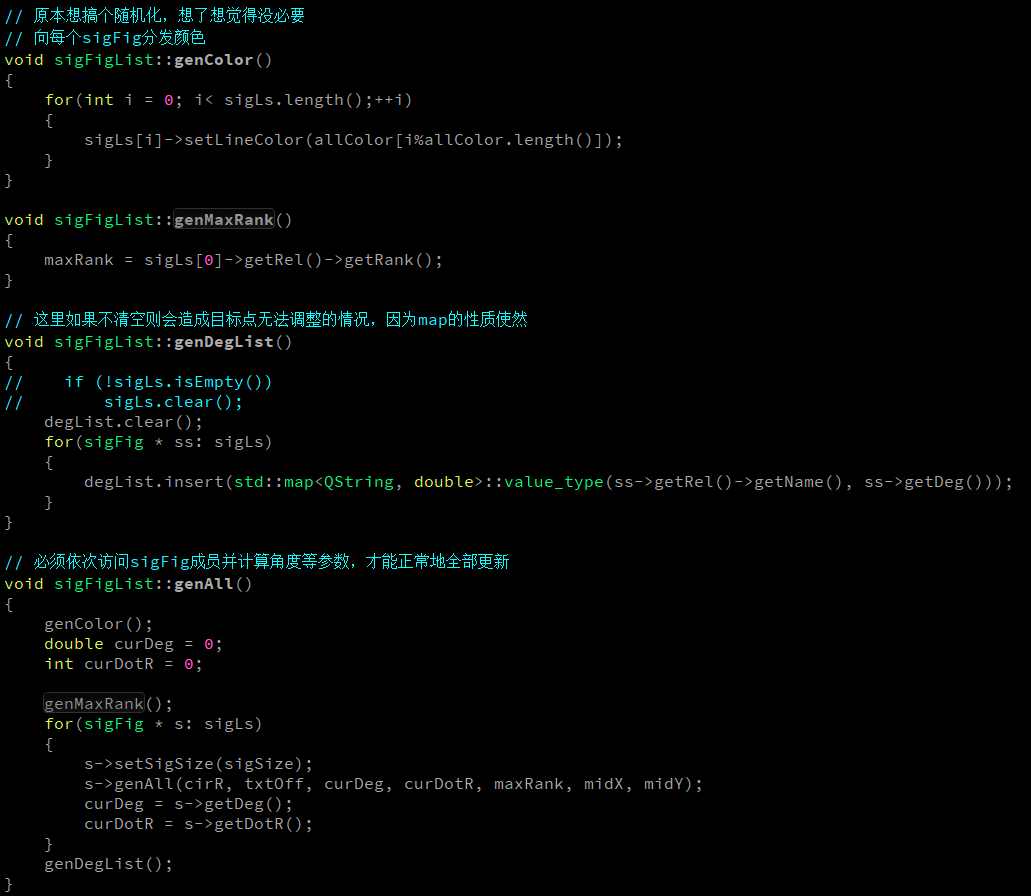
\includegraphics[width = 15cm]{task6-sigFigList.png}
    \caption{分发颜色、更新角度列表、更新疏密程度具体实现}
    \label{task6-sigFigList}
\end{figure}

\par mainwindow 类:
\par 对画布上产生的各类信号给出对应的槽进行处理,具体的任务交给
fgLs去做。如载入文件、设置显示个数以及疏密程度的滚动条、鼠标移动
设置高亮的判断等。如图\ref{task6-mainwindow}
\begin{figure}[htbp]
    \centering
    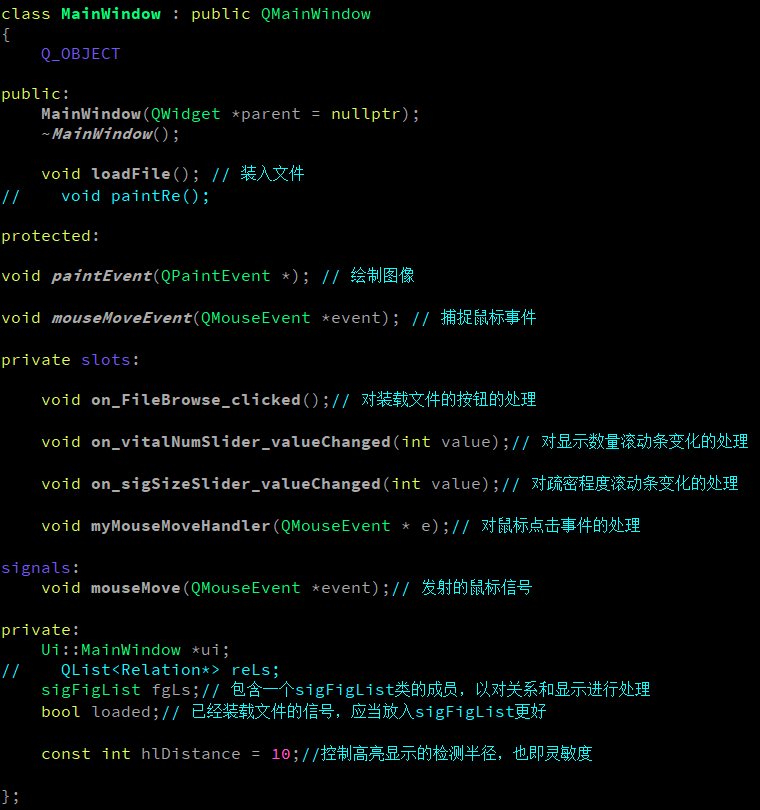
\includegraphics[width = 15cm]{task6-mainwindow.png}
    \caption{mainwindow具体实现}
    \label{task6-mainwindow}
\end{figure}

\subsubsection{结果展示}
\begin{figure}[htbp]
    \centering
    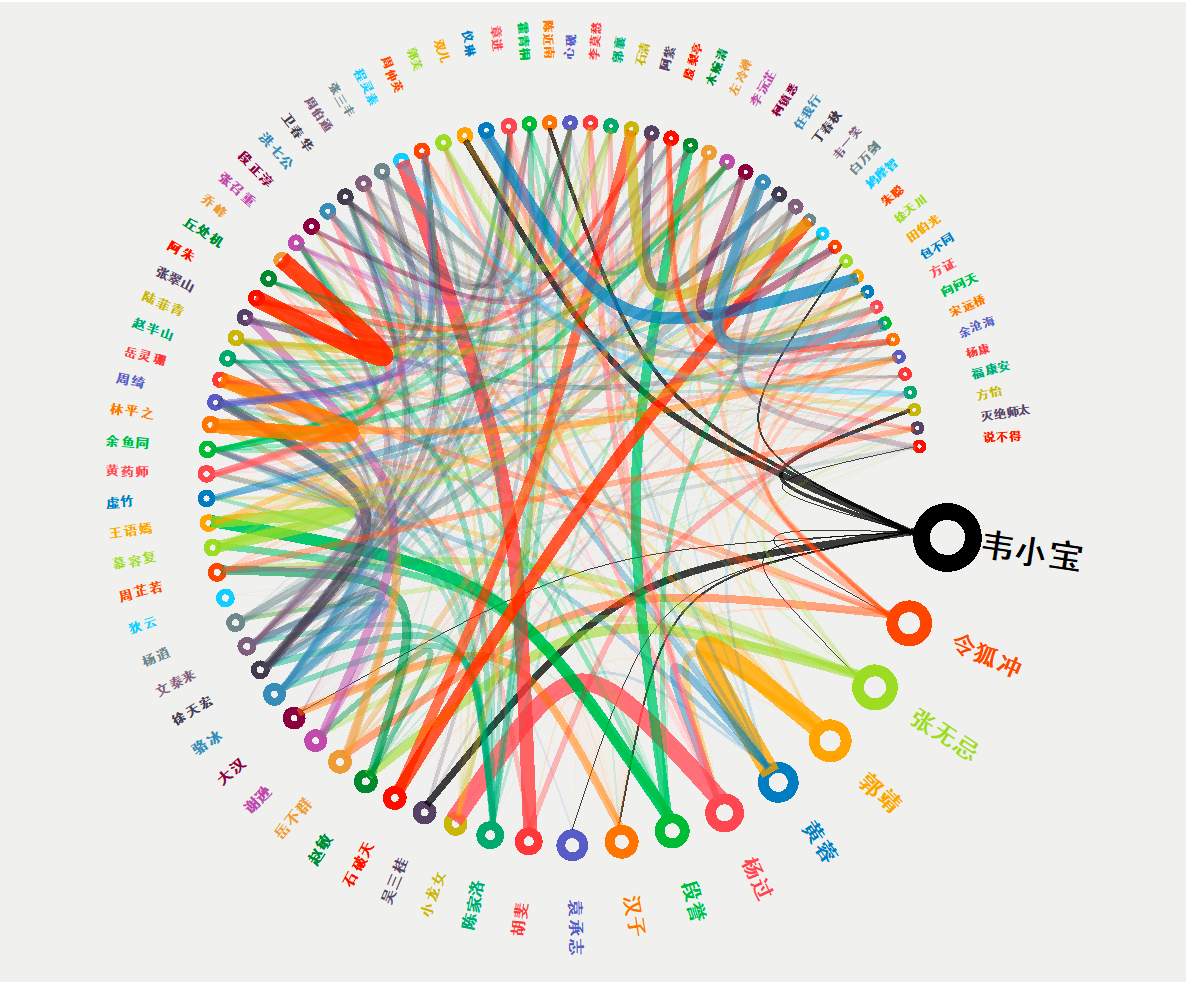
\includegraphics[width = 15cm]{task6-result.png}
    \caption{可视化结果}
    \label{task6-result}
\end{figure}
如图\ref{task6-result}打开程序,导入文件并调整滚动条至合适位置,
可以看到最重要的n位人物及其关系列表出现在屏幕
中央。几条最粗的曲线彰显了郭靖与黄蓉、杨过与小龙女、
胡斐与程灵素、慕容复与王语嫣、张无忌与周芷若
等等人物之间的密切关系。通过不同的颜色,可以相对容易地查找与同一人物相关的人物关系。
\par 必要时,可以调整人物关系颜色透明度,并拖动鼠标更改高亮人物,从而获取
更高质量的信息。
\begin{figure}[htbp]
    \centering
    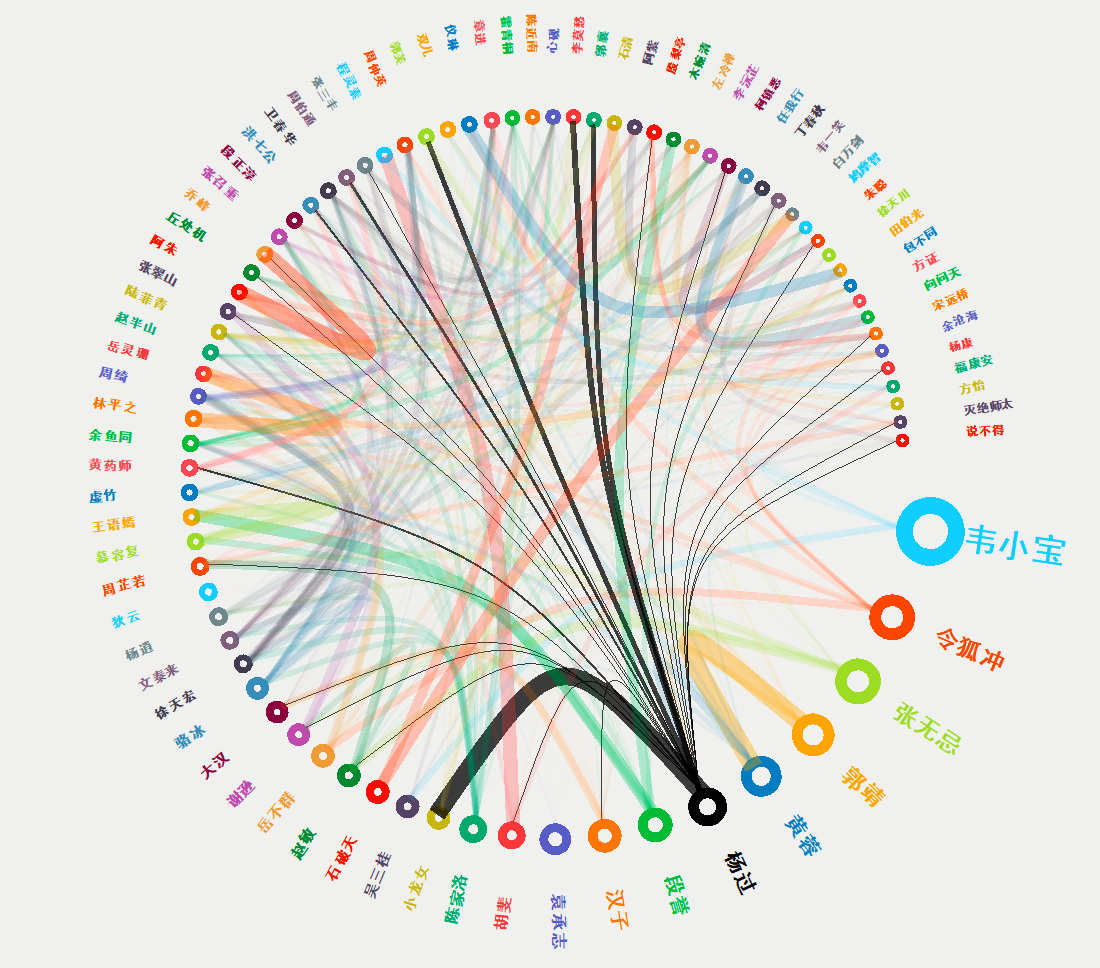
\includegraphics[width = 15cm]{task6-result2.png}
    \caption{透明度调整与高亮效果}
    \label{task6-result2}
\end{figure}
如图\ref{task6-result2},通过调整透明度与高亮人物,
可以清晰地看到杨过的人物关系。

\section{优化与改进}
\subsection{任务二}
\begin{itemize}
    \item 数据格式中很多地方使用Text传输。可以考虑使用自定义Writable数据格式,来减少序列化时间和传输损耗。
    \item 统计人物同现时,可以考虑根据人物字母顺序,
    将<a,b>与<b,a>统一为<a,b>。这样任务二mapper和reducer之间
    减少一倍的传输损耗,任务二的输出结果将减少一倍占用空间,
    任务三mapper读、任务二reducer写也将减少一倍读写文件时间损耗。
    实现时可以将任务二mapper中HashSet用TreeSet代替来保证有序,
    在内部for循环中只发射在外部for循环当前值之后(或之前)的部分。
    当然任务三中mapper就要修改为:既发射第一个人名又发射第二个人名。
    之后保持不变。当然也要考虑到TreeSet比HashSet可能要消耗更多时间。
\end{itemize}

\subsection{任务三}
reducer中HashMap的使用是没有必要的。应该使用类似List<Pair<String, Integer>>代替,加快reducer端时间、空间效率。

\subsection{任务四}
\begin{enumerate}[1)]
    \item 原本迭代次数为20次,在检查中间结果时发现在14次之后,结果变化不大,基本收敛,因此将迭代次数改为15次,节省时间开销。
    \item 完整版的PageRank计算会引入随机跳转,避免自环节点以及无出度节点导致无法收敛。而本次数据实际不存在此类节点,因此无需引入,节省计算量。
    \item PageRank算法原本RP值设置为访问概率1/N,这样结果值为各节点的概率,和为1。但本次实验我们注重的是人物之间的相对重要程度,因此将PR放大N倍,设置初始值为1.0,从而以减小小数运算误差。
\end{enumerate}
\subsection{任务五}
LPA当遇到二分图的时候,会出现标签震荡,这里当迭代轮数超过 10 轮后就会开始震荡,因此我们这里可以选择迭代 15 -20轮。
通过对实验五的结果进行分析,我们可以看出,相同标签的人物都是在同一本书中的人物。但因为人物同现关
系窗口选择的大小问题,会出现一些很小的簇或者孤岛
\subsection{任务六}
\begin{enumerate}[1)]
    \item 【已经优化】由于QPainter的绘制特性缘故,因此人物的姓名有一半是倒着的,造成观感不佳,需要解决。
    \item 【已经优化】 由于曲线使用点集绘制,而单点的绘制被自动设置为方形,因此曲线的形状不佳,需要改进。
    \item 【已经优化】由于曲线使用的颜色的亮度、深浅不同,造成人物关系密切程度的直观性降低,需要改进颜色组。
    \item 采用数据结构效率较低,对于冗余的判断和循环没有进行优化,造成操作上的延迟,需要优化。
    \item 由于采用的是高Rank值的人物向低Rank值的人物绘制曲线,因此造成低rank值人物
    快速无法快速辨认全部与其相关的人物关系。可以采用颜色的渐变进行优化。
    \item 尚存在很多绘制参数没有在外部留出接口,例如透明度无法在用户界面设置,需要改进。
\end{enumerate}

\section{Hadoop集群执行报告及结果展示}
\subsection{执行指令}
\subsubsection{任务一}
\begin{figure}[H]
    \centering
    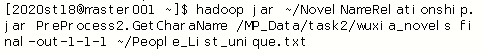
\includegraphics[width = 15cm]{task1-1-input.png}
    \caption{任务一指令}
\end{figure}

\subsubsection{任务二}
\begin{figure}[H]
    \centering
    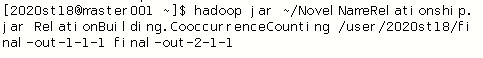
\includegraphics[width = 15cm]{task2-1-input.png}
    \caption{任务二指令}
\end{figure}

\subsubsection{任务三}
\begin{figure}[H]
    \centering
    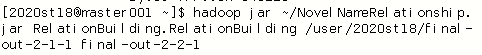
\includegraphics[width = 15cm]{task3-1-input.png}
    \caption{任务三指令}
\end{figure}

\subsubsection{任务四}
\begin{figure}[H]
    \centering
    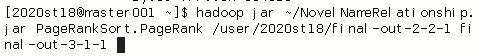
\includegraphics[width = 15cm]{task4-1-input.png}
    \caption{任务四指令1}
\end{figure}
\begin{figure}[H]
    \centering
    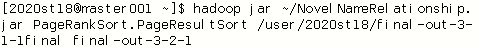
\includegraphics[width = 15cm]{task4-2-input.png}
    \caption{任务一指令2}
\end{figure}

\subsubsection{任务五}
\begin{figure}[H]
    \centering
    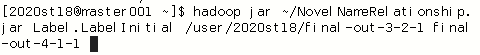
\includegraphics[width = 15cm]{task5-1-input.png}
    \caption{任务五指令1}
\end{figure}
\begin{figure}[H]
    \centering
    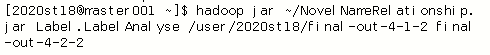
\includegraphics[width = 15cm]{task5-2-input.png}
    \caption{任务五指令2}
\end{figure}
\begin{figure}[H]
    \centering
    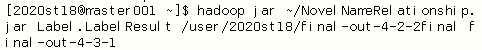
\includegraphics[width = 15cm]{task5-3-input.png}
    \caption{任务五指令3}
\end{figure}

\subsection{WebUI}
\subsubsection{任务一}
\begin{figure}[H]
    \centering
    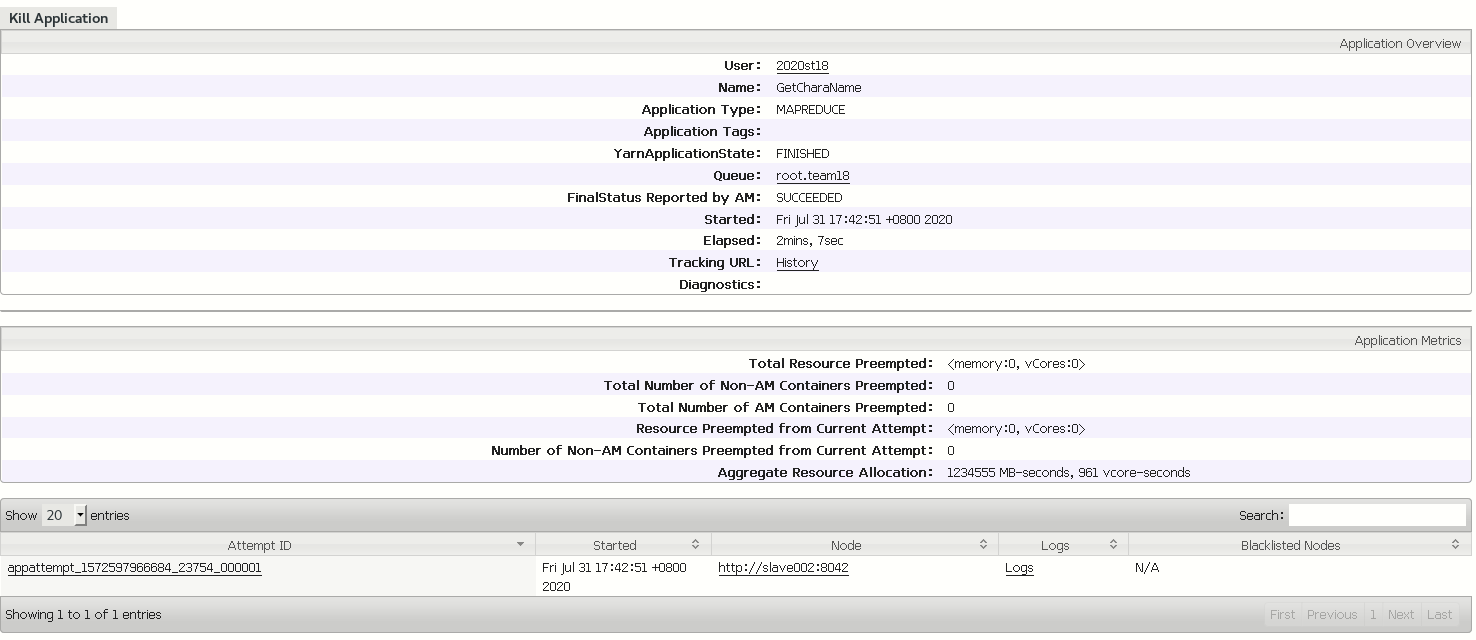
\includegraphics[width = 15cm]{task1-1-success.png}
    \caption{任务一WebUI}
\end{figure}

\subsubsection{任务二}
\begin{figure}[H]
    \centering
    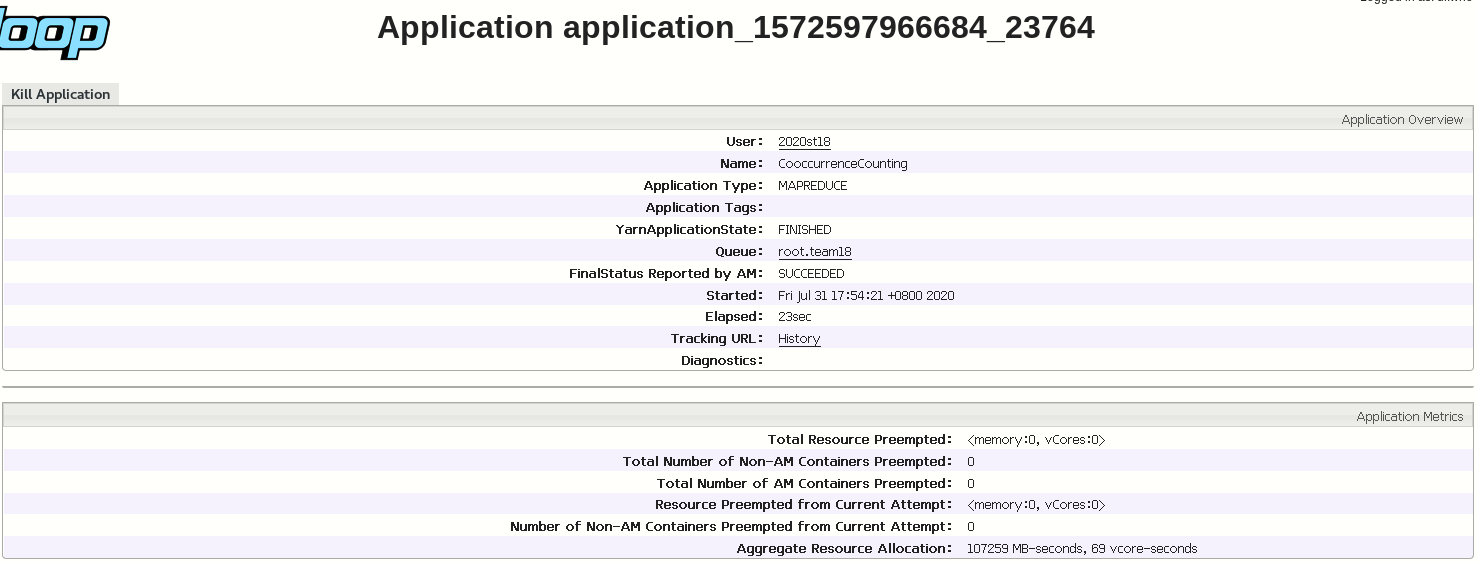
\includegraphics[width = 15cm]{task2-1-success.png}
    \caption{任务二WebUI}
\end{figure}

\subsubsection{任务三}
\begin{figure}[H]
    \centering
    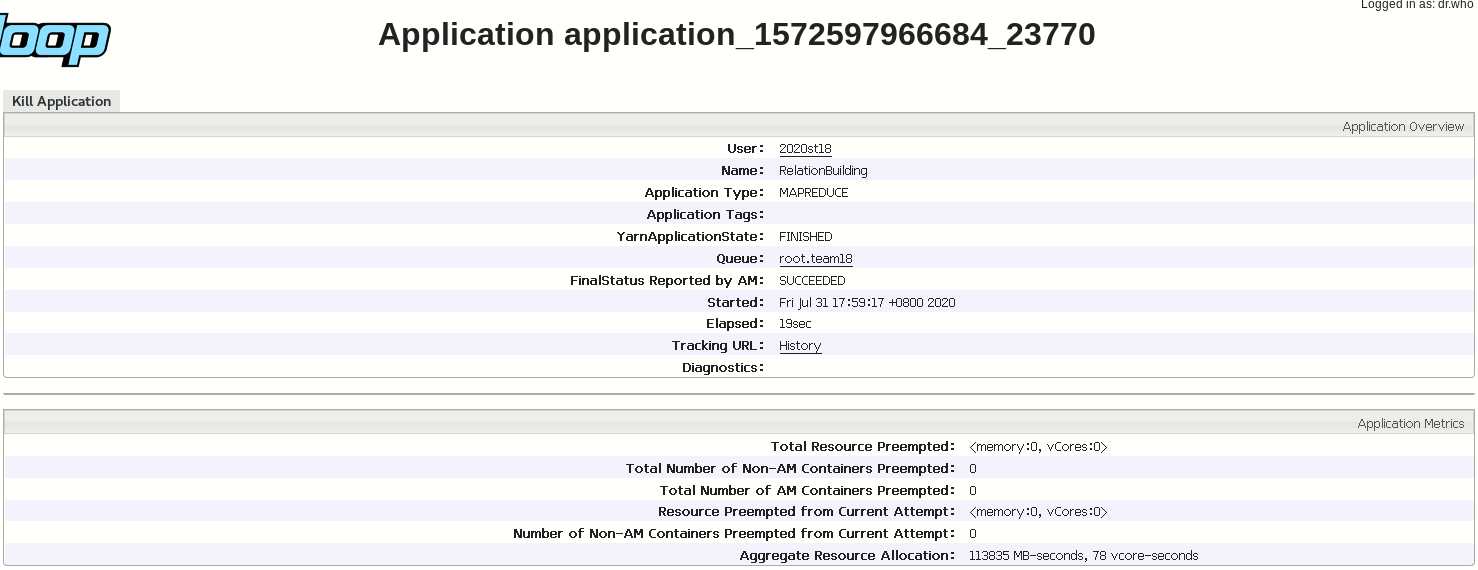
\includegraphics[width = 15cm]{task3-1-success.png}
    \caption{任务三WebUI}
\end{figure}

\subsubsection{任务四}
\begin{figure}[H]
    \centering
    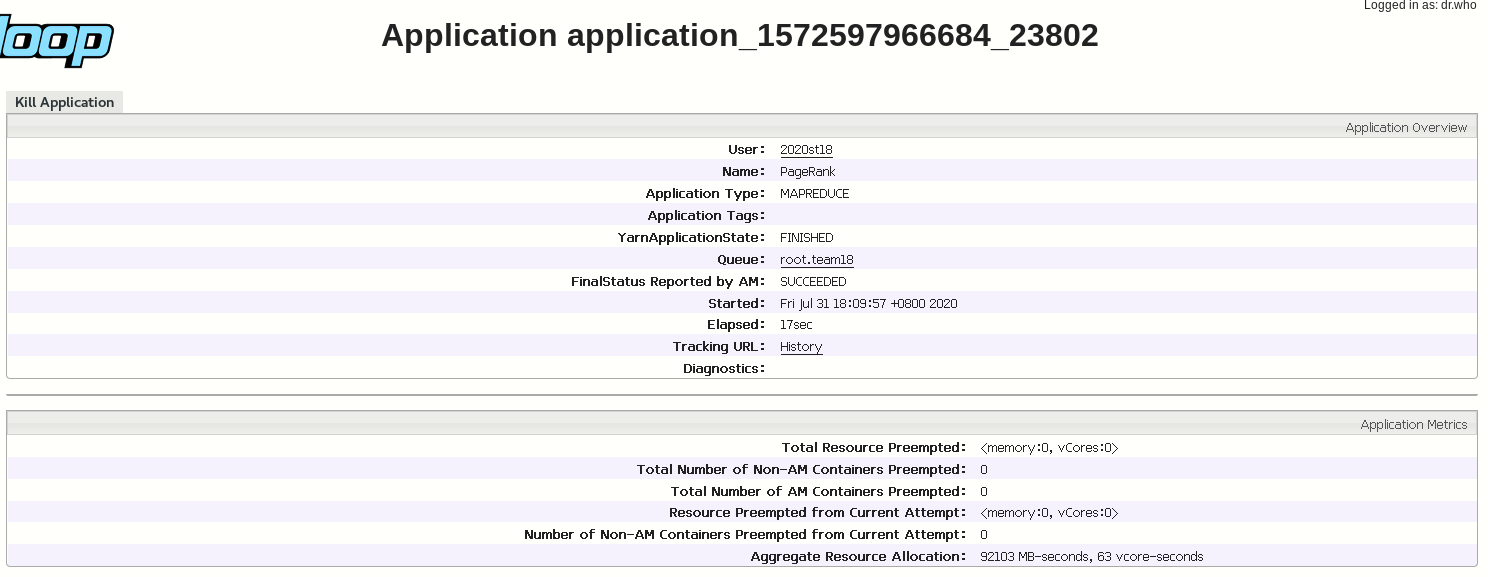
\includegraphics[width = 15cm]{task4-1-success.png}
    \caption{任务四WebUI1}
\end{figure}
\begin{figure}[H]
    \centering
    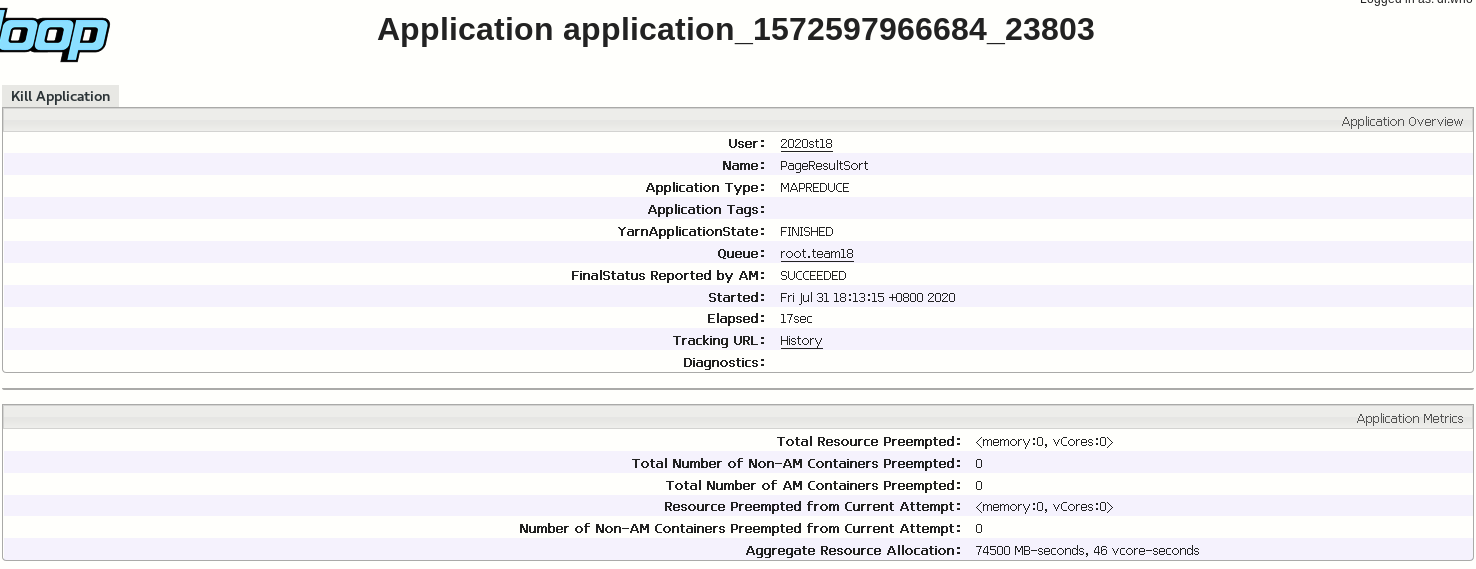
\includegraphics[width = 15cm]{task4-2-success.png}
    \caption{任务四WebUI2}
\end{figure}

\subsubsection{任务五}
\begin{figure}[H]
    \centering
    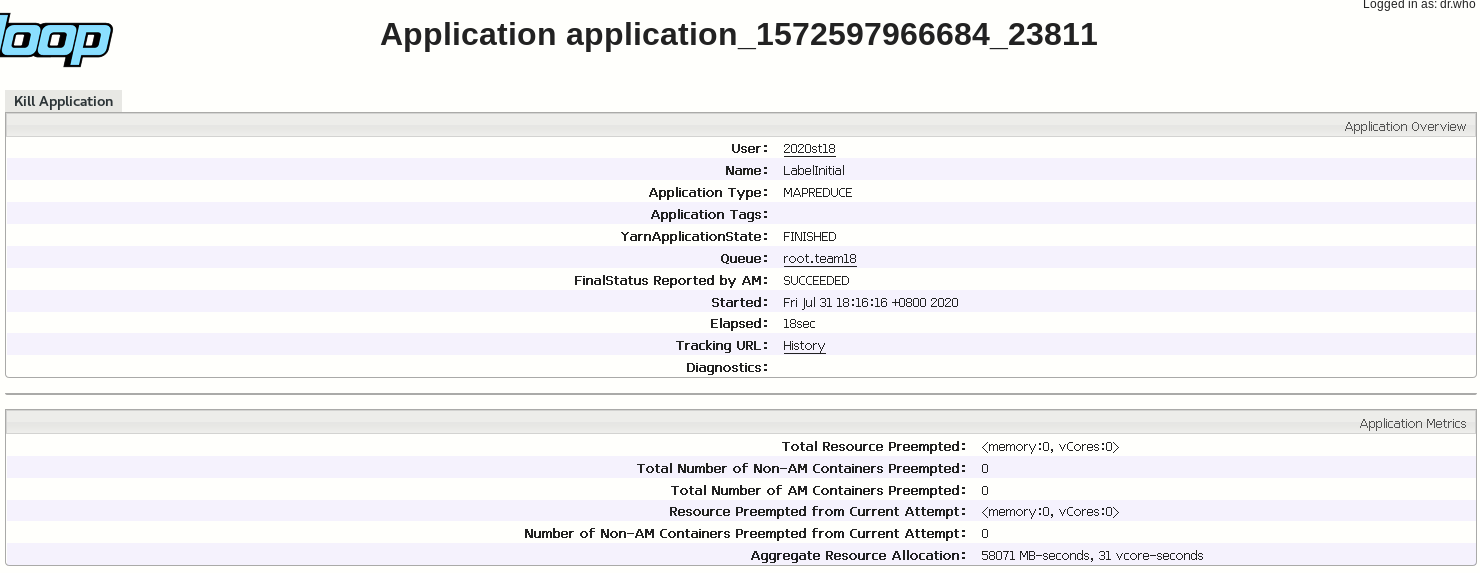
\includegraphics[width = 15cm]{task5-1-success.png}
    \caption{任务五WebUI1}
\end{figure}
\begin{figure}[H]
    \centering
    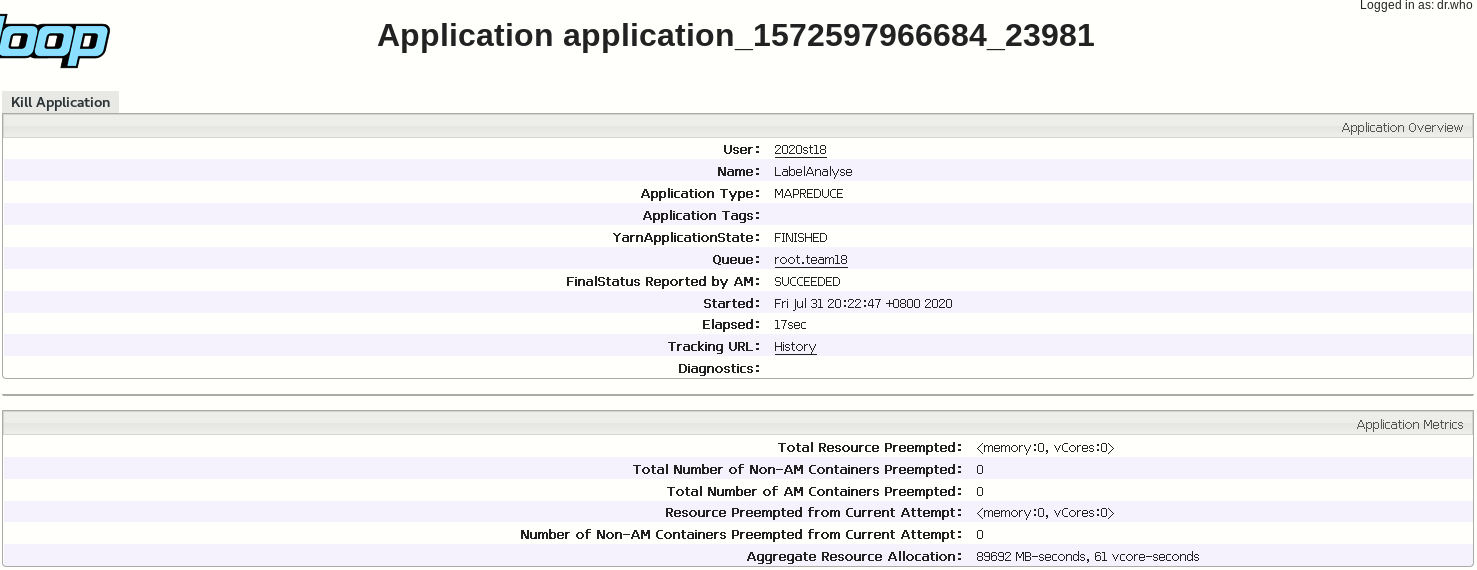
\includegraphics[width = 15cm]{task5-2-success.png}
    \caption{任务五WebUI2}
\end{figure}
\begin{figure}[H]
    \centering
    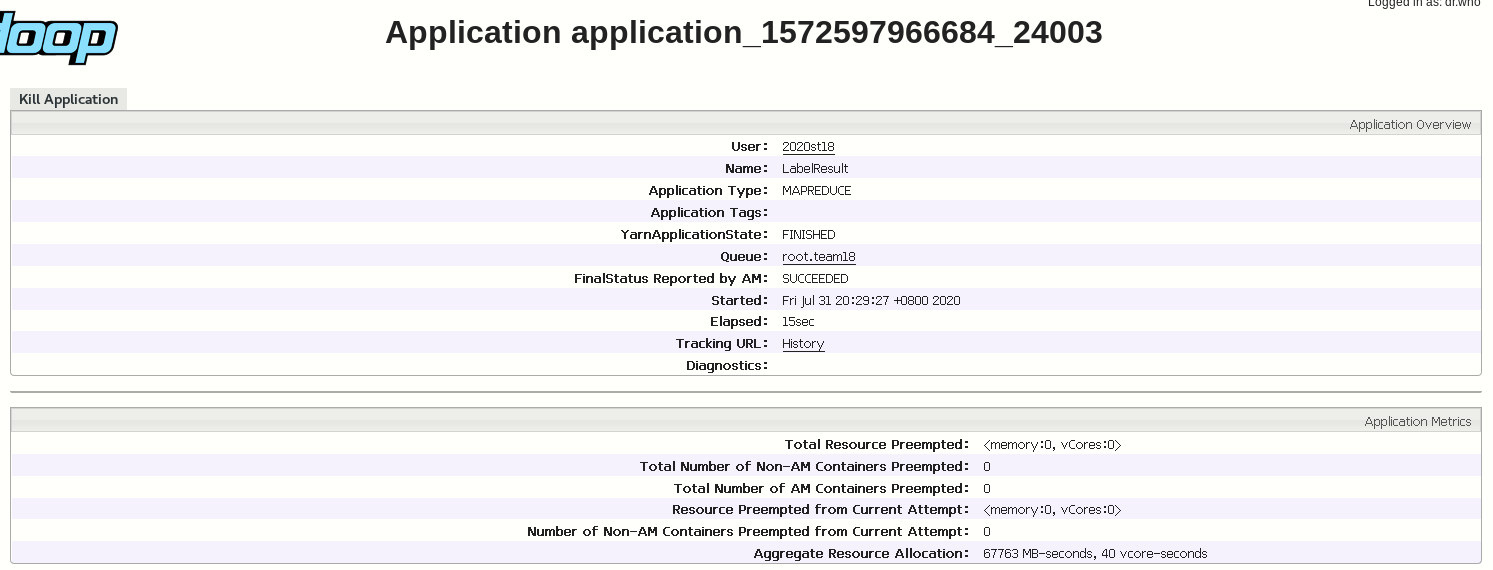
\includegraphics[width = 15cm]{task5-3-success.png}
    \caption{任务五WebUI3}
\end{figure}

\subsection{部分结果展示}
\subsubsection{任务一}
\begin{figure}[H]
    \centering
    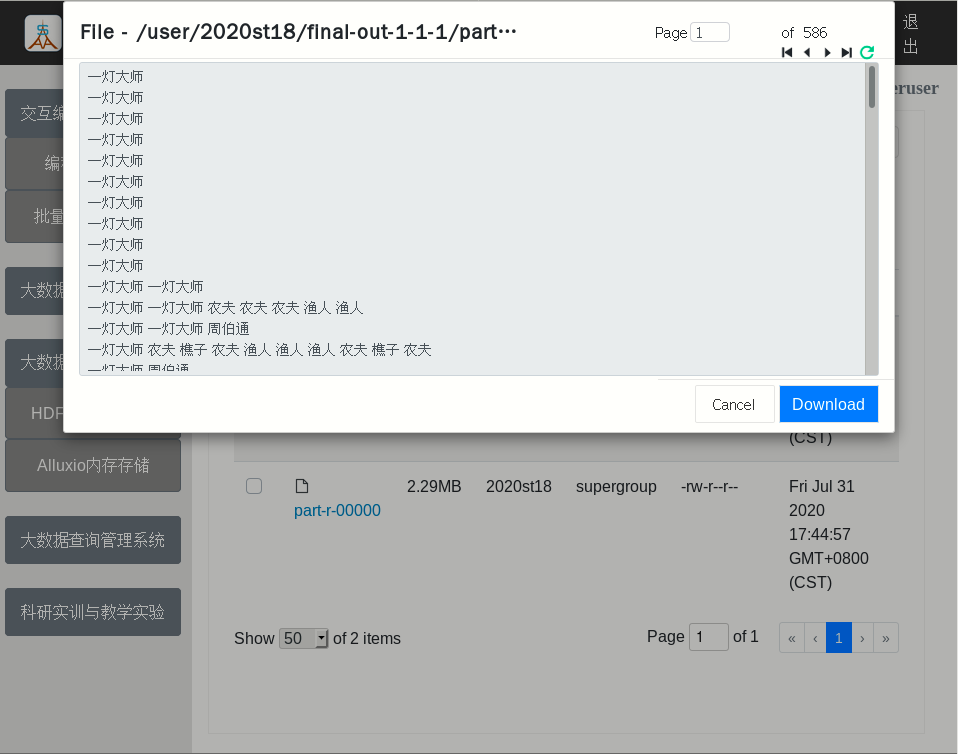
\includegraphics[width = 15cm]{task1-1-output.png}
    \caption{任务一结果}
\end{figure}

\subsubsection{任务二}
\begin{figure}[H]
    \centering
    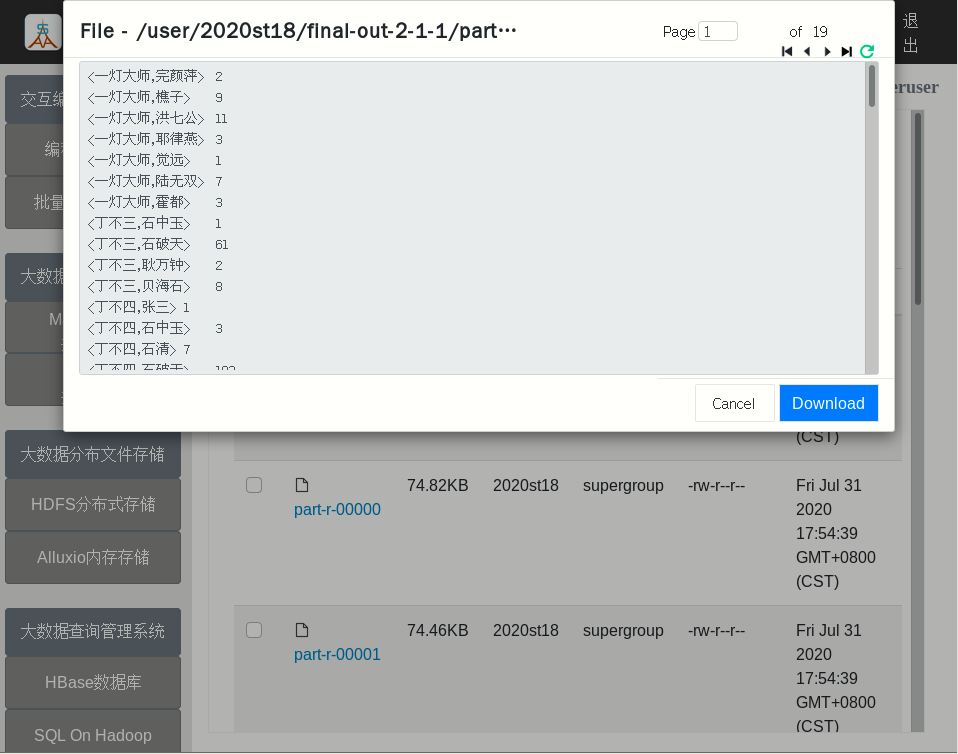
\includegraphics[width = 15cm]{task2-1-output.png}
    \caption{任务二结果}
\end{figure}

\subsubsection{任务三}
\begin{figure}[H]
    \centering
    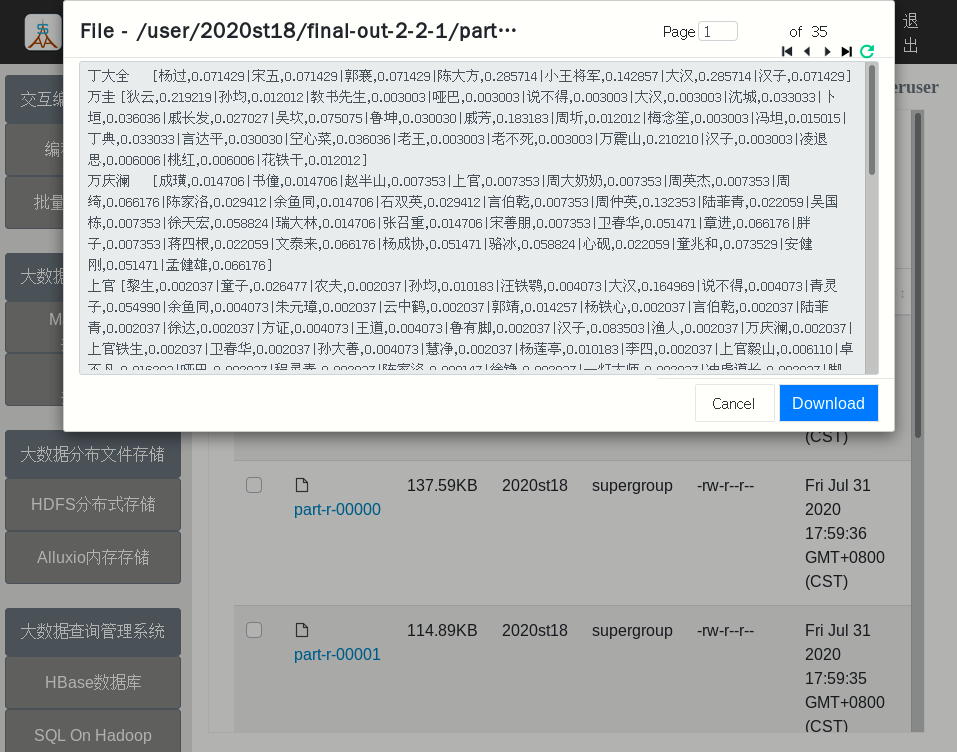
\includegraphics[width = 15cm]{task3-1-output.png}
    \caption{任务三结果}
\end{figure}

\subsubsection{任务四}
\begin{figure}[H]
    \centering
    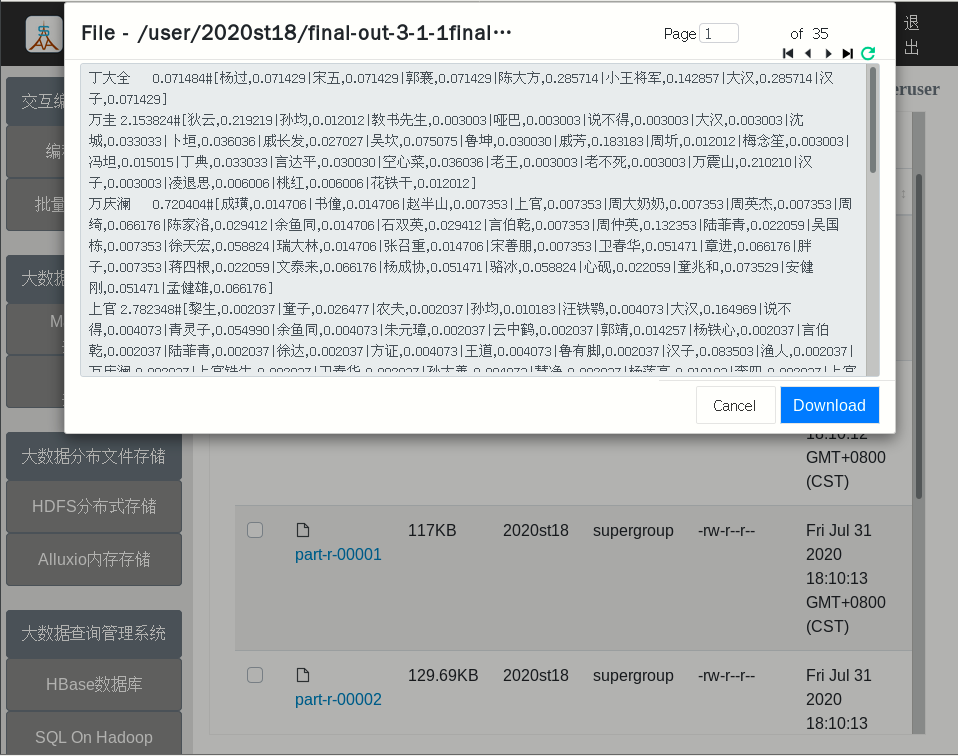
\includegraphics[width = 15cm]{task4-1-output.png}
    \caption{任务四结果1}
\end{figure}
\begin{figure}[H]
    \centering
    \includegraphics[width = 15cm]{task4-2-output.png}
    \caption{任务四结果2}
\end{figure}

\subsubsection{任务五}
\begin{figure}[H]
    \centering
    \includegraphics[width = 15cm]{task5-1-output.png}
    \caption{任务五结果1}
\end{figure}
\begin{figure}[H]
    \centering
    \includegraphics[width = 15cm]{task5-2-output.png}
    \caption{任务五结果2}
\end{figure}
\begin{figure}[H]
    \centering
    \includegraphics[width = 15cm]{task5-3-output.png}
    \caption{任务五结果3}
\end{figure}


\bibliographystyle{plain}
\bibliography{ref}

\end{document}
